\newcommand{\DoNotLoadEpstopdf}{}
\documentclass[11pt,a4paper]{article}
\ifdefined\pdfinfoomitdate\pdfinfoomitdate=1\fi
\ifdefined\pdftrailerid\pdftrailerid{}\fi
\ifdefined\pdfsuppressptexinfo\pdfsuppressptexinfo=15\fi
\input{glyphtounicode-cmex}
\pdfgentounicode=1
\usepackage[T1]{fontenc}
\usepackage{lmodern}
\usepackage[margin=29mm]{geometry}
\usepackage{amsmath,amssymb,amsthm,mathtools}
\usepackage{microtype}
\usepackage{enumitem}
\usepackage{xcolor}
\usepackage{tikz}
\usetikzlibrary{arrows.meta,positioning}
\usepackage[colorlinks=true,linkcolor=blue!45!black,citecolor=blue!45!black,
urlcolor=blue!45!black,bookmarksnumbered=true]{hyperref}
\newcommand{\R}{\mathbb R}
\newcommand{\C}{\mathbb C}
\newcommand{\PP}{\mathbb P}
\newcommand{\Z}{\mathbb Z}
\newcommand{\cO}{\mathcal O}
\newcommand{\dd}{\mathrm d}
\newcommand{\id}{\mathrm{id}}
\DeclareMathOperator{\Ham}{Ham}
\DeclareMathOperator{\vol}{vol}
\DeclareMathOperator{\Bl}{Bl}
\DeclareMathOperator{\Int}{int}
\DeclareMathOperator{\supp}{supp}
\DeclareMathOperator{\pr}{pr}
\newcommand{\sq}{\mathbin{\sqcup}}
\newcommand{\eps}{\varepsilon}
\newcommand{\pair}[2]{\langle #1,#2\rangle}
\newcommand{\norm}[1]{\left\lVert #1\right\rVert}
\newtheorem{theorem}{Theorem}[section]
\newtheorem{lemma}[theorem]{Lemma}
\newtheorem{proposition}[theorem]{Proposition}
\newtheorem{corollary}[theorem]{Corollary}
\theoremstyle{definition}
\newtheorem{definition}[theorem]{Definition}
\theoremstyle{remark}
\newtheorem{remark}[theorem]{Remark}
\numberwithin{equation}{section}
\setlist[enumerate]{itemsep=3pt,topsep=6pt}
\setlist[itemize]{itemsep=3pt,topsep=6pt}
\hypersetup{pdftitle={Symplectic Ball Packings in Higher Dimensions},
pdfsubject={A proof of the Siegel--Yao ball-packing conjecture},
pdfauthor={OpenAI}}

\title{Symplectic Ball Packings in Higher Dimensions}
\author{OpenAI}
\date{September 23, 2026}
\begin{document}
\maketitle
\begin{abstract}
We prove that, for all integers \(n\ge3\) and \(k\ge1\) and all
positive real capacities \(R_1,\ldots,R_k\), the closed standard
symplectic \(2n\)-balls of these capacities embed disjointly into the interior
of a ball of capacity \(R>0\) if and only if
\[
 \sum_{i=1}^k R_i^n<R^n,
 \qquad R_i+R_j<R\quad(i\ne j).
\]
Capacity is \(\pi\) times the squared Euclidean radius, and each
embedding is defined on a neighborhood of its closed source ball.
This proves Siegel and Yao's Conjecture~A.
\end{abstract}
\begingroup
\small
\tableofcontents
\endgroup
\section{Introduction}\label{intro:section}

Symplectic ball packing asks how much of a volume-preserving embedding
problem is constrained by symplectic rigidity. For \(R>0\), write
\[
 B^{2n}(R)=
 \left\{z\in\C^n:\pi\sum_{j=1}^n|z_j|^2\le R\right\},
 \qquad
 \omega_0=\sum_{j=1}^n\dd x_j\wedge\dd y_j.
\]
Thus \(R\) is the capacity, the Euclidean radius is \(\sqrt{R/\pi}\),
and \(\vol B^{2n}(R)=R^n/n!\). We ask when finitely many such balls
can be embedded symplectically into the interior of a target ball.
An embedding of a closed ball is understood to be a symplectic embedding
defined on an open neighborhood of it. For a finite disjoint union, the
compact images of the closed balls must be pairwise disjoint.

\begin{theorem}\label{intro:main}
Let \(n\ge3\) and \(k\ge1\) be integers. For positive real numbers
\(R,R_1,\ldots,R_k\), there exists a symplectic embedding
\[
 \bigsqcup_{i=1}^k B^{2n}(R_i)
 \hookrightarrow \Int B^{2n}(R)
\]
if and only if
\begin{equation}\label{intro:inequalities}
 \sum_{i=1}^k R_i^n<R^n,
 \qquad
 R_i+R_j<R\quad (1\le i<j\le k).
\end{equation}
\end{theorem}

The first inequality is the volume obstruction. The second is Gromov's
two-ball obstruction~\cite{Gromov1985}; it expresses a restriction
invisible to volume alone. Theorem~\ref{intro:main} proves that these
obstructions are complete in every real dimension at least six, resolving
Siegel and Yao's Conjecture~A positively~\cite{SiegelYao2025}. For one
ball the pairwise condition is vacuous. The strict inequalities reflect
the closed-source, open-target convention.

\subsection{Packing rigidity and stability}

Gromov's pseudoholomorphic-curve method gives the two-ball obstruction
in every dimension, and further packing obstructions in dimension
four~\cite[Section~0.3.B]{Gromov1985}. McDuff and Polterovich developed
the connection with algebraic geometry~\cite{McDuffPolterovich}.
Explicit constructions form a complementary strand: Traynor developed
symplectic packing constructions~\cite{Traynor}, and Schlenk developed
planar constructions and higher-dimensional folding
methods~\cite{SchlenkHand,SchlenkBook}. In real dimension four,
additional obstructions remain essential, so the two inequalities in
Theorem~\ref{intro:main} do not give a criterion there.

Biran's work~\cite{Biran1997,Biran1999} established packing stability:
on a closed symplectic four-manifold with rational symplectic class,
every sufficiently large number of equal balls can fill an arbitrarily
large fraction of the volume. Buse and Hind extended equal-ball
stability to higher-dimensional balls and projective spaces and then to all closed
rational symplectic manifolds~\cite{BuseHind2011,BuseHind2013}.
For unequal balls, Buse, Hind, and Opshtein proved strong packing
stability on every closed symplectic four-manifold, with all capacities
required to be sufficiently small~\cite{BuseHindOpshtein2016}.
These results identify regimes in which volume suffices; the question
here concerns every finite collection of arbitrary capacities in a ball.

Siegel and Yao formulate this higher-dimensional question and also study
stabilized packing problems~\cite{SiegelYao2025}. Their theorems on
products of four-dimensional balls with a fixed closed symplectic surface
retain four-dimensional packing obstructions. Theorem~\ref{intro:main}
concerns balls themselves, with arbitrary unequal capacities and
arbitrary finite numbers of components.

\subsection{From a mean area inequality to ball embeddings}

Normalize the target capacity to one. The common construction uses a
surface of positive genus as a base and a toric domain in \(\C^m\),
where \(m=n-1\), as a fiber. The fiber is specified by a downward
polytope \(\Delta\subset\R_{\ge0}^m\) in the moment coordinates
\(p_j=\pi|z_j|^2\): lowering any coordinate keeps a point in
\(\Delta\). Write \(H(p)>0\) for the limiting total area of the
base at fixed moment \(p\), obtained by exhausting a punctured
surface by compact bordered pieces. A ball of auxiliary capacity
\(r_i\), chosen strictly larger than the corresponding requested
capacity, requires the area profile
\[
\left(r_i-\sum_{j=1}^m p_j\right)_+,
 \qquad x_+=\max(x,0).
\]
The models contain each auxiliary simplex \(\sum_jp_j\le r_i\)
strictly away from their noncoordinate boundary faces.
The volume inequality becomes positivity of the integral of the
unused-area profile
\[
 P(p)=H(p)-\sum_i\left(r_i-\sum_jp_j\right)_+
\]
over \(\Delta\). This integral condition need not make \(P\) positive
at each moment, which is the obstacle to simply stacking the balls.

Section~\ref{cmp:section} overcomes that obstacle by Hamiltonian
comparison. Under concavity of \(P\) and positivity outside a radial
core of \(\Delta\), Lemma~\ref{cmp:comparison} constructs a smooth
toric function \(K\) and a Hamiltonian map \(q\) such that
\[
 (K-P)\circ q<K.
\]
Coordinatewise increasing rearrangements of convex functions preserve
their integrals and lead to a contraction whose fixed point gives a
uniform gap. Smooth planar disk maps realize the rearrangements with
errors smaller than that gap. Near each noncoordinate boundary face,
the generating Hamiltonians commute with its defining moment function;
this is the boundary control needed in the next step.

Section~\ref{surf:section} converts the comparison into embeddings.
A handle provides two transverse annuli and a closed one-form with a
nonzero period. These allow the Hamiltonian change of fiber coordinates
to be inserted into an exact symplectic deformation. The uniform gap
leaves disjoint layers whose area profiles contain the requested balls.
The relative Moser argument in Lemma~\ref{surf:packing} returns the
packing to the original model, preserving its boundary conditions.
The construction uses the limiting concave function \(P\); the
integrated areas of finite bordered models need only converge uniformly.

The connection between packing and Hamiltonian-group structure described
in Edtmair's abstracts~\cite{EdtmairPerfectness2025,EdtmairPacking2025}
was one motivation for the commutator viewpoint in this construction.
The present one-handle comparison and exact deformation are constructed
locally, rather than obtained from those results.

\subsection{The geometric models and the three cases}

To apply this mechanism we need models carrying nearly all the available
volume over a surface with a handle. The use of a polarization to expose
standard symplectic regions has precedents in Biran's decomposition
method~\cite{Biran2001} and Opshtein's singular polarizations and
ellipsoid packings~\cite{Opshtein2013}. Witt Nystr\"om showed that modified
deformations to the normal cone can place arbitrarily nearly all the
volume of a compact K\"ahler manifold in a normal-bundle
component~\cite{WittNystrom2024}. Here explicit toric models over
positive-genus curves supply the area profiles needed by the surface
packing lemma. Section~\ref{geo:devices} develops the relative transfer
statements that take compact packings from these models back to the
target. Its deformation and reduction tools are Moser's
method~\cite{Moser1965}, symplectic cuts~\cite{Lerman1995}, and their
K\"ahler interpretation~\cite{BurnsGuilleminLerman2002}; the relative and
equivariant details are proved where needed.

The pairwise inequalities leave three cases, summarized in
Figure~\ref{fig:proof-flow}. If every requested capacity is below
\(1/2\), Section~\ref{app:applications} degenerates \(\PP^n\)
along a complete intersection of quadrics. Its curve has positive genus
for every \(n\ge3\), and its normal model approaches the full volume
of the target. Proposition~\ref{app:small} applies the surface packing
lemma to this model.

If a requested capacity is at least \(1/2\), it is the unique such
capacity. Reserve a slightly larger central ball and pack the remaining
balls into its exterior shell. For \(n\ge4\), a hyperplane degeneration
followed by a curve degeneration in its base gives a positive-genus model
of that shell. This is Proposition~\ref{app:large}, also in
Section~\ref{app:applications}.

In complex dimension three, the same procedure would use a plane conic,
which has genus zero. Section~\ref{six:section} instead starts from a
quadric through the blowup point and uses a further degeneration along
a plane cubic with two marked points. If the reserved capacity is
\(a>1/2\), set \(s=1-a\) and \(b=(2-a)/3\). The resulting
integrated base area is
\[
 H_0(p)=9(b-p_1-p_2)-2(s-p_1-p_2)_+.
\]
Each marked point contributes one of the two subtracted logarithmic
masses. This concave density gives the required shell volume, while
exact preservation of the first circle moment \(p_1\) under transport
permits a lower
K\"ahler cut. The cubic family also supplies the invariant K\"ahler
form needed for that cut. Proposition~\ref{six:large} completes this
last case, and Section~\ref{app:completion} assembles the theorem.

All requested capacities remain arbitrary positive real numbers.
Rational auxiliary polarizations and compact truncations are chosen
with strict slack. Every transfer is defined on a neighborhood of the
relevant compact set, so the construction retains embeddings of the
whole closed source balls under finite composition.

\begin{figure}[tbp]
\centering
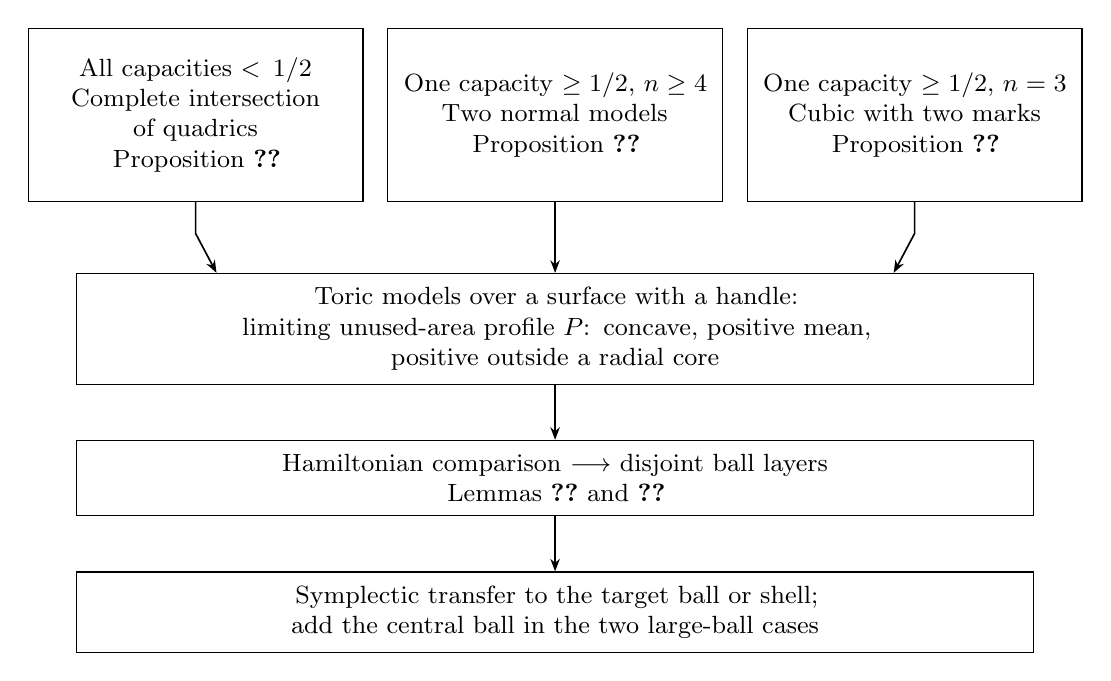
\begin{tikzpicture}[
  font=\small,
  box/.style={draw,align=center,inner sep=5pt,text width=39mm,minimum height=22mm},
  wide/.style={draw,align=center,inner sep=5pt,text width=118mm},
  arr/.style={-{Stealth[length=1.6mm]},semithick}]
 \node[box] (small) {All capacities \(<1/2\)\\
   Complete intersection\\of quadrics\\Proposition~\ref{app:small}};
 \node[box,right=3mm of small] (large) {One capacity \(\ge1/2\), \(n\ge4\)\\
   Two normal models\\Proposition~\ref{app:large}};
 \node[box,right=3mm of large] (six) {One capacity \(\ge1/2\), \(n=3\)\\
   Cubic with two marks\\Proposition~\ref{six:large}};
 \node[wide,below=9mm of large] (model) {Toric models over a surface with a handle:\\
   limiting unused-area profile \(P\): concave, positive mean,\\
   positive outside a radial core};
 \node[wide,below=7mm of model] (packing) {Hamiltonian comparison
   \(\longrightarrow\) disjoint ball layers\\
   Lemmas~\ref{cmp:comparison} and~\ref{surf:packing}};
 \node[wide,below=7mm of packing] (target) {Symplectic transfer to the target ball or shell;\\
   add the central ball in the two large-ball cases};
 \draw[arr] (small.south) -- ++(0,-4mm) -- ([xshift=-43mm]model.north);
 \draw[arr] (large) -- (model);
 \draw[arr] (six.south) -- ++(0,-4mm) -- ([xshift=43mm]model.north);
 \draw[arr] (model) -- (packing);
 \draw[arr] (packing) -- (target);
\end{tikzpicture}
\caption{The three geometric applications feed the same comparison and
surface-packing mechanism. Capacities are normalized by the target
capacity. The six-dimensional transfer also uses the lower K\"ahler cut.
The one-ball case is immediate.}
\label{fig:proof-flow}
\end{figure}


\subsection{Conventions and the easy direction}

We use the Hamiltonian convention
\(\iota_{X_H}\omega=-\dd H\). On \(\C^m\), moment and angle coordinates
are
\[
 p_j=\pi|z_j|^2,\qquad
 \theta_j=\frac{\arg z_j}{2\pi},\qquad
 \omega_0=\sum_j\dd p_j\wedge\dd\theta_j.
\]
Moment formulas are always interpreted in the original smooth complex
coordinates at a coordinate axis. A function is \emph{toric} if it
depends only on the moments. Projective spaces and line bundles use
Chern class units: a projective line in the unit class has area one.
Projectivizations parametrize lines, and \(U=c_1(\cO(1))\) denotes the
dual tautological class. We normalize \(\dd^c\) by
\(\dd^c\log|z|^2=\dd\theta\) away from zero; consequently
\(\dd\dd^c\log|z|^2\) has a unit atom at zero.

\begin{proof}[Necessity in Theorem~\ref{intro:main}]
The union of the finitely many compact images is contained in
\(\Int B^{2n}(\sigma)\) for some \(\sigma<R\).
Volume preservation gives
\(\sum_iR_i^n\le\sigma^n<R^n\). Gromov's two-ball obstruction
\cite[Section~0.3.B]{Gromov1985}, in the capacity convention
of~\cite[Theorem~1.1]{SiegelYao2025}, gives
\(R_i+R_j\le\sigma<R\) for every pair.
\end{proof}

Conjugating the source and target by the same dilation reduces
sufficiency to target capacity one; the conformal factors in the two
pullbacks cancel. We henceforth use this normalization. A single ball
of capacity less than one embeds by inclusion. The proof for multiple
balls is completed after the three geometric applications, in
Section~\ref{app:completion}.

\section{Hamiltonian comparison on a toric domain}\label{cmp:section}

Our goal is to turn a positive mean area surplus into a strict
pointwise inequality after a Hamiltonian change of fiber coordinates.
The construction must also preserve the boundary moments needed by
the surface deformation in Section~\ref{surf:section}.

Let
\begin{equation}\label{cmp:polytope}
 \Delta=\{p\in\R_{\ge0}^m:
             b_\nu\cdot p\le c_\nu,\ 1\le\nu\le N\},
 \qquad b_\nu\in\R_{\ge0}^m,\quad c_\nu>0,
\end{equation}
be compact and full dimensional, with \(m\ge1\).
We call the nonempty faces \(b_\nu\cdot p=c_\nu\) the
\emph{outer faces}. The coordinate faces \(p_j=0\) are not outer faces.
Put
\[
 V=\{z\in\C^m:p(z)\in\Delta\},\qquad
 p_j(z)=\pi|z_j|^2,
\]
with its standard symplectic form \(\omega_V\).
We freely regard functions on \(\Delta\) as toric functions on \(V\).
Smooth maps, Hamiltonians, and differential forms on these compact
sets will always be defined on neighborhoods. No simplicity or
rationality assumption on \(\Delta\) is needed.

\begin{lemma}[Hamiltonian comparison]\label{cmp:comparison}
Let \(P:\Delta\to\R\) be continuous and concave. Suppose that its
Lebesgue mean \(\overline P\) is positive and, for some \(0<\tau<1\),
\begin{equation}\label{cmp:outer-positive}
 \inf_{\Delta\setminus\tau\Delta}P>0.
\end{equation}
Then there are a smooth toric function \(K\) and a Hamiltonian
diffeomorphism \(q:V\to V\) such that
\begin{equation}\label{cmp:conclusion}
 (K-P)(qu)<K(u)\qquad(u\in V).
\end{equation}
The map \(q\) admits a Hamiltonian isotopy from the identity preserving
\(V\), whose Hamiltonians Poisson commute with \(b_\nu\cdot p\) near
each corresponding outer face, uniformly in time.
\end{lemma}

We separate the rearrangement inequality from its symplectic realization.
First we define the rearrangement operator and state the realization
property needed by the proof.  The fixed-point argument then produces a
uniform gap; the remaining subsection proves the realization property
with an arbitrarily small error and the required boundary control.

\subsection{Coordinate rearrangements}

For a continuous convex function \(f:[0,1]\to\R\), its increasing
rearrangement with respect to Lebesgue measure at \(h\in[0,1]\)
can be written as
\begin{equation}\label{cmp:interval-formula}
 g(h)=\min_{0\le a\le1-h}\max\{f(a),f(a+h)\}.
\end{equation}
This also defines the endpoint values \(g(0)=\min f\) and
\(g(1)=\max f\).

For a continuous convex function \(F\) on \(\Delta\), let \(R_jF\)
denote increasing rearrangement in \(p_j\), with the other moments
\(y=(p_i)_{i\ne j}\) fixed. The slice is \([0,L(y)]\), where
\[
 L(y)=
 \min_{\nu:b_{\nu j}>0}
 \frac{c_\nu-\sum_{i\ne j}b_{\nu i}y_i}{b_{\nu j}}.
\]
At least one such bound exists by compactness of \(\Delta\).
The function \(L\) is continuous, concave, and piecewise affine
on the projected polytope. Define \(R_jF\) by the rescaled version
of~\eqref{cmp:interval-formula}.

\begin{lemma}\label{cmp:rearrangement-properties}
Each \(R_j\) maps continuous convex functions on \(\Delta\) to
continuous convex functions. It preserves Lebesgue integrals,
order, and addition of constants, and is nonexpansive in uniform
norm. Its output is nondecreasing in \(p_j\); moreover it preserves
being nondecreasing in any other coordinate.
Consequently \(R=R_m\cdots R_1\) has coordinatewise nondecreasing
output.
\end{lemma}

\begin{proof}
Continuity follows from the minimum-over-intervals formula. At a
slice of length tending to zero, uniform continuity of \(F\) gives
the same conclusion. For convexity, choose minimizing intervals
of lengths \(h_0,h_1\) on two slices. Their convex combination is
an allowed interval of length \((1-t)h_0+th_1\) on the intermediate
slice. Convexity of \(F\) bounds its two endpoint values by the
corresponding convex combinations, which proves convexity of
the rearrangement.

The minimum formula is nondecreasing in the interval length.
If \(F\) is nondecreasing in another coordinate, lowering that
coordinate preserves every allowed interval, by the nonnegative
coefficients in~\eqref{cmp:polytope}, and can only lower its
endpoint values. This proves preservation of the previous
monotonicity properties.

On each slice, increasing rearrangement preserves the distribution
of values, including flat sublevels, and hence the integral.
Integrate this identity in the other coordinates.
Order and translation invariance follow directly from the
minimum formula. Applying these to
\(G-\norm{F-G}_\infty\le F\le G+\norm{F-G}_\infty\)
proves nonexpansiveness.
\end{proof}

The following lemma realizes one coordinate rearrangement up to a prescribed
error.  Its proof, given after the proof of Lemma~\ref{cmp:comparison},
uses smooth families of planar disk maps.

\begin{lemma}[Lifted rearrangement]\label{cmp:lifted}
For every continuous convex \(F:\Delta\to\R\), every coordinate \(j\),
and every \(\eps>0\), there is a Hamiltonian diffeomorphism
\(q_j:V\to V\) such that
\[
 F\circ q_j\le R_jF+\eps.
\]
Its isotopy preserves \(V\), and its Hamiltonians Poisson commute
with every outer-face moment near the corresponding face.
\end{lemma}

\subsection{A fixed point with a uniform gap}

\begin{proof}[Proof of Lemma~\ref{cmp:comparison}]
The continuous convex functions on \(\Delta\) form a complete
metric space in the uniform norm. Since \(-P\) is convex,
Lemma~\ref{cmp:rearrangement-properties} implies that, for
\(0<\lambda<1\), the map
\[
 F\longmapsto R(\lambda F-P)
\]
is a contraction of this space, with constant \(\lambda\).
Let \(K_\lambda\) be its fixed point. Integral preservation gives
\begin{equation}\label{cmp:mean}
 \overline K_\lambda
 =-\frac{\overline P}{1-\lambda}.
\end{equation}
The function \(K_\lambda\) is coordinatewise nondecreasing;
in particular \(K_\lambda(0)=\min_\Delta K_\lambda\).

Choose
\[
 0<d<\min\left\{\overline P,\,
               \inf_{\Delta\setminus\tau\Delta}P\right\}.
\]
We claim that, for \(\lambda\) sufficiently close to one,
\begin{equation}\label{cmp:negative-maximum}
 M_\lambda:=\max_\Delta K_\lambda
 <-\frac d{1-\lambda}.
\end{equation}
Suppose otherwise for such a \(\lambda\).
Then \(\lambda M_\lambda\le M_\lambda+d\), and consequently
\(\lambda K_\lambda-P<M_\lambda\) on the outer region.
For \(p\in\tau\Delta\), write \(p=\tau v\) with \(v\in\Delta\).
Convexity, \(K_\lambda(0)\le\overline K_\lambda\), and
\eqref{cmp:mean} give
\[
 K_\lambda(p)
 \le \tau M_\lambda-
       \frac{(1-\tau)\overline P}{1-\lambda}
 \le M_\lambda-
       \frac{(1-\tau)(\overline P-d)}{1-\lambda}.
\]
It follows that
\[
 \lambda K_\lambda(p)-P(p)
 \le M_\lambda+d
 -\frac{\lambda(1-\tau)(\overline P-d)}{1-\lambda}
 -\min_\Delta P<M_\lambda
\]
when \(\lambda\) is close enough to one. The choices here depend
only on the displayed constants, so the bound is uniform on
both regions. We have shown
\(\max_\Delta(\lambda K_\lambda-P)<M_\lambda\), contradicting
the fixed-point equation and
\(\max RF\le\max F\). This proves
\eqref{cmp:negative-maximum}.

Fix such a \(\lambda\). Since
\((1-\lambda)K_\lambda\le-d\), order preservation and
translation invariance give
\begin{equation}\label{cmp:rearranged-gap}
 R(K_\lambda-P)
 \le R(\lambda K_\lambda-P)-d=K_\lambda-d.
\end{equation}
Set \(F_0=K_\lambda-P\) and \(F_j=R_jF_{j-1}\).
All these functions are continuous and convex.
Use Lemma~\ref{cmp:lifted} to choose \(q_j\) with
\[
 F_{j-1}\circ q_j\le F_j+\eps_j,
 \qquad \sum_j\eps_j<d/2.
\]
In the order \(q=q_1\circ\cdots\circ q_m\), successive
substitution of these inequalities yields
\[
 (K_\lambda-P)\circ q
 \le R(K_\lambda-P)+\sum_j\eps_j
 <K_\lambda-d/2.
\]
Each constituent isotopy preserves \(V\) and preserves every
outer-face moment on a sufficiently small collar.
Choose common threshold collars
\(c_\nu-\epsilon_\nu< b_\nu\cdot p\le c_\nu\)
for the finitely many maps.
Such collars are invariant because the moment is constant
along each flow there. Run the isotopy for \(q_m\) first, then that for \(q_{m-1}\)
on its output, and continue in this order. Each stage uses one of
the original generating Hamiltonians and retains its commutation
with every face moment. Reparametrization makes the concatenated
path smooth and preserves these commutation relations.

Finally approximate \(K_\lambda\) uniformly on \(\Delta\) by
a smooth function \(K(p)\), defined on a neighborhood.
Polynomial approximation is sufficient.
An approximation error smaller than \(d/4\) changes the last
comparison by less than \(d/2\), leaving
\((K-P)\circ q<K\). This proves the lemma.
\end{proof}

\subsection{Realization by Hamiltonian maps}

We now prove the realization lemma used above.  Related constructions
prescribe planar symplectic maps by nested equal-area curves;
see \cite[Lemma~3.2]{SchlenkFolding}.  We need smooth parameter
dependence and relative Hamiltonian control as well.

Write \(D(A)=\{z\in\C:\pi|z|^2<A\}\).
A smooth family of embedded closed disks means a family of smooth
embeddings of the closed unit disk, smooth also in the parameters on
an open neighborhood of their parameter set.

\begin{lemma}[Nested disks]\label{cmp:planar-disks}
Let \(Y\) be a compact convex subset of a Euclidean space, let
\(0<a_1<\cdots<a_l<A\), and let
\[
 E_1(y)\Subset\Int E_2(y)\Subset\cdots
       \Subset\Int E_l(y)\Subset D(A)
 \qquad(y\in Y)
\]
be smooth families of embedded closed disks of areas \(a_1,\ldots,a_l\).
There is a smooth family of Hamiltonian isotopies of \(D(A)\),
supported in a common compact subset, whose endpoint maps carry each
centered disk of area \(a_j\) onto \(E_j(y)\).
\end{lemma}

\begin{proof}
First construct ordinary orientation-preserving diffeomorphisms with
these properties. At a fixed parameter \(y_0\), a disk embedding can
be shrunk within its image, straightened while small, moved through
the ambient disk, and expanded to another prescribed disk. The
velocity along its moving boundary extends to a vector field in a
tubular neighborhood and then, by a cutoff, to a compactly supported
ambient field. The resulting flow extends the disk isotopy.
Apply this construction first to the outermost boundary and then to
each successive boundary inside its already positioned outer disk.
This gives a compactly supported diffeomorphism \(\phi_{y_0}\),
isotopic to the identity, carrying the centered disks to the prescribed
ones.

For other parameters, follow the disk boundaries along the segment
\(y_0+t(y-y_0)\). Their velocities extend in disjoint tubular
neighborhoods of the finitely many boundaries. These extensions can
be chosen smoothly in \((t,y)\), by local extensions and a partition
of unity. Compactness and strict nesting give uniform collars and
support away from the ambient boundary. Integrating the fields
produces diffeomorphisms \(\phi_y\), with ordinary isotopies smooth in
\(y\), carrying all the centered disks to their prescribed images.

Let \(\omega\) be the standard area form and
\(\eta_y=\phi_y^*\omega-\omega\).
This is a compactly supported two-form of integral zero.
Compactly supported primitives can be chosen linearly, and hence
smoothly in \(y\). For completeness, identify the open ambient disk
smoothly with \(\R^2\), write \(\eta=f(x,t)\,\dd x\wedge\dd t\),
and choose a fixed compactly supported function \(\rho\) with
\(\int\rho=1\). Put
\[
 g(t)=\int_\R f(x,t)\,\dd x,\quad
 F(x,t)=\int_{-\infty}^x\bigl(f(v,t)-\rho(v)g(t)\bigr)\,\dd v,
 \quad G(t)=\int_{-\infty}^t g(v)\,\dd v.
\]
Then
\[
 \alpha=F\,\dd t-\rho(x)G(t)\,\dd x,\qquad
 \dd\alpha=\eta.
\]
The zero marginal and zero total integral give compact support, with
a common support for compact families.

For every centered disk \(D_j\) of area \(a_j\),
\[
 \int_{D_j}\eta_y
 =\operatorname{area}E_j(y)-a_j=0.
\]
Thus the restriction of \(\alpha_y\) to \(\partial D_j\) is exact.
Subtract the differentials of functions extending these circle
primitives into disjoint annular collars. The resulting primitive
\(\widehat\alpha_y\) vanishes on the tangent line of each circle.
Apply Moser's method~\cite{Moser1965} to
\(\omega+t\eta_y\), \(0\le t\le1\), using
\(\widehat\alpha_y\). This path consists of positive area forms.
Its vector fields are tangent to the designated circles, since
\(\widehat\alpha_y\) vanishes on their tangents. The resulting
correction \(\chi_y\) preserves every \(D_j\) and satisfies
\(\chi_y^*\phi_y^*\omega=\omega\).
Hence \(\psi_y=\phi_y\circ\chi_y\) is area preserving and has the
required disk images.

It remains to provide a symplectic isotopy with this endpoint.
The construction has already supplied an ordinary compactly
supported isotopy \(\psi_{y,t}\) from the identity to \(\psi_y\).
For each \((y,t)\), apply the same Moser correction, now without
circle conditions, to
\[
 \omega+s(\psi_{y,t}^*\omega-\omega),\qquad 0\le s\le1.
\]
Use the linear primitive operator above. When
\(\psi_{y,t}^*\omega=\omega\), that primitive and the correction are
zero and the identity, respectively. In particular, the corrections
are the identity at both endpoints \(t=0,1\). The corrected isotopy
is therefore symplectic, has endpoint \(\psi_y\), and is smooth in
the parameters. On a disk, a compactly supported symplectic vector
field has a Hamiltonian normalized to vanish on the complementary
component adjacent to the ambient boundary. These Hamiltonians depend
smoothly on the parameters and are supported in a common larger compact
subset of the disk. This yields the required Hamiltonian isotopies.
\end{proof}

\begin{lemma}[Planar rearrangement]\label{cmp:disk-realization}
Let \(f_y:[0,1]\to\R\) be a jointly continuous family of convex
functions, with \(y\) in a compact convex parameter set. Let \(g_y\)
be their increasing rearrangements with respect to Lebesgue measure.
For every \(\eps>0\), there is a smooth family of compactly supported
Hamiltonian isotopies of \(D(1)\), with endpoints \(\psi_y\), such that
\[
 f_y\bigl(\pi|\psi_y(z)|^2\bigr)
 \le g_y(\pi|z|^2)+\eps
 \qquad(z\in\overline{D(1)}).
\]
Their supports lie in a common compact subset of \(D(1)\).
\end{lemma}

\begin{proof}
The minimum formula~\eqref{cmp:interval-formula} shows that
\(g_y(h)\) is jointly continuous in \((y,h)\).

Choose a small \(\eps'>0\) and a sufficiently fine grid
\(0<h_1<\cdots<h_l<1\), including points sufficiently close to both
endpoints. The open intervals
\[
 I_j(y)=
 \{v\in(0,1):f_y(v)<g_y(h_j)+\eps'\}
\]
are nested in \(j\), and each has length greater than \(h_j\).
Indeed, the closed sublevel at \(g_y(h_j)\) contains an interval
of length \(h_j\), and the strict enlargement gives extra room.
Joint continuity and compactness make this room uniform for the
finite grid.

Choose increasing numbers \(w_j<1\), sufficiently close to one, so
that \(h_j/w_j\) is strictly increasing in \(j\) and is smaller than
the available length of \(I_j(y)\) for every \(y\).
There are strictly nested closed intervals \(J_j(y)\), of lengths
\(h_j/w_j\), contained in \(I_j(y)\). To choose them, first choose
the smallest interval and enlarge successively inside the next
available open interval. The admissible centers satisfy strict
affine inequalities expressing containment and nesting. Locally
constant admissible centers remain admissible near a given
parameter. A smooth partition of unity preserves these convex
constraints, and therefore gives centers smooth on a neighborhood
of the parameter set.

In the open polar chart \((v,\theta)\in(0,1)^2\), take the rectangles
\[
 J_j(y)\times
 \left[\frac{1-w_j}{2},\frac{1+w_j}{2}\right].
\]
Their areas are \(h_j\). Round the corners smoothly and adjust the
width in the \(v\)-direction slightly to restore the area exactly.
For example, superellipses of a common sufficiently large even
exponent approximate all these rectangles, and their areas are
corrected by one additional dilation in \(v\).
The strict margins ensure that the resulting smooth closed disks
\(E_j(y)\) remain nested and lie in \(I_j(y)\times(0,1)\).
All choices are uniform because the parameter set and grid are
compact and finite.

Apply Lemma~\ref{cmp:planar-disks} to these disks. If \(v\le h_j\),
the image of a point of radial area \(v\) lies in \(E_j(y)\), and
therefore its \(f_y\)-value is below \(g_y(h_j)+\eps'\).
Use the next larger grid point and uniform continuity of \(g_y\)
to bound this by \(g_y(v)+2\eps'\).
For \(v>h_l\), use
\(f_y\le\max f_y=g_y(1)\) and choose \(h_l\) close enough to one.
Taking \(\eps'\) small proves the assertion. The Hamiltonians
extend by zero across the ambient boundary, so the same inequality
holds on the closed disk.
\end{proof}

\begin{proof}[Proof of Lemma~\ref{cmp:lifted}]
First suppose that a slice has a smooth positive area scale
\(\ell(y)\). Apply Lemma~\ref{cmp:disk-realization} to
\(f_y(v)=F(y,\ell(y)v)\).
If \(B_t(y,z)\) generates the resulting maps on \(D(1)\), then
the Hamiltonian
\[
 \ell(y)B_t\bigl(y,z_j/\sqrt{\ell(y)}\bigr)
\]
on the whole fiber produces the desired scaled disk motion.
The other moments remain fixed because this Hamiltonian has no
dependence on their angles. Their angles may change, which does
not affect a toric function.

To treat the actual endpoint \(L\), choose a small \(\eta>0\) and
work first on the compact convex parameter set
\[
 Y_\eta=\{y:L(y)\ge\eta\}.
\]
Choose a smooth function \(\ell\) strictly below \(L\), uniformly
close to it on \(Y_\eta\), and with \(\ell\ge\eta/2\).
For instance, a smooth soft minimum of the finitely many affine
expressions defining \(L\), shifted downward by a small positive
constant, has these properties when its approximation error is small.
The planar construction and its
Hamiltonians extend smoothly to a neighborhood of \(Y_\eta\).

For \(h\le\ell(y)\), any interval of length \(h\) in \([0,L(y)]\)
can be shifted into \([0,\ell(y)]\) by a distance at most
\(L(y)-\ell(y)\). Hence, for a uniform modulus of continuity
\(\omega_F\),
\begin{equation}\label{cmp:shortened-slice}
 R_{[0,\ell]}F(h)
 \le R_{[0,L]}F(h)+\omega_F(L-\ell).
\end{equation}
For \(\ell<h\le L\), let \([a,a+h]\) be a minimizing interval
for the right-hand rearrangement. Since \(a\le L-h<L-\ell\),
\begin{equation}\label{cmp:outer-strip}
 F(y,h)\le R_{[0,L]}F(h)+\omega_F(L-\ell).
\end{equation}
Thus the identity map in this outer strip has the required
one-sided estimate. The planar Hamiltonians vanish near their
rescaled boundary, so this identity extension is smooth.

Choose a smooth cutoff \(0\le\chi(y)\le1\), supported where
\(L>\eta\) and equal to one where \(L\ge2\eta\), with its support
contained in the neighborhood where the preceding choices are
defined. The full lifted Hamiltonian is
\begin{equation}\label{cmp:cutoff-hamiltonian}
 \chi(y)\ell(y)
 B_{\chi(y)t}\bigl(y,z_j/\sqrt{\ell(y)}\bigr),
 \qquad 0\le t\le1,
\end{equation}
extended by zero elsewhere. At fixed \(y\), it runs the scaled
disk isotopy to time \(\chi(y)\). On slices of length at most
\(2\eta\), any slice-preserving motion incurs error at most
\(\omega_F(2\eta)\), since all slice values of \(F\) have that
oscillation bound. Elsewhere \(\chi=1\), and
\eqref{cmp:shortened-slice}--\eqref{cmp:outer-strip}, together
with the planar estimate, apply. Choose \(\eta\), the scale
error, and the planar error in this order to make the total
error less than \(\eps\).

All lifts are smooth at the other coordinate axes because
the other moments are smooth functions of the complex variables.
The cutoff removes the possible degeneracy at \(L=0\).
To check the outer faces, suppose first that \(b_{\nu j}>0\).
Equality on that face forces \(p_j=L(y)\). On active slices the
common compact planar support satisfies
\[
 p_j\le(1-\delta)\ell(y)
\]
for some \(\delta>0\), while \(\ell(y)\ge\eta/2\).
Writing \(L_\nu(y)\) for this face's affine endpoint, its support
therefore satisfies
\[
 c_\nu-b_\nu\cdot p
 =b_{\nu j}(L_\nu(y)-p_j)
 \ge b_{\nu j}\delta\ell(y)
 \ge b_{\nu j}\delta\eta/2>0.
\]
Thus the Hamiltonian vanishes on a genuine uniform neighborhood
of that face. If \(b_{\nu j}=0\), the Hamiltonian commutes with
\(b_\nu\cdot p\) everywhere. These statements imply that the
flow preserves all defining inequalities of \(V\) and gives
the stated face property.
\end{proof}

\section{Packing over a surface with a handle}\label{surf:section}

The comparison lemma becomes a packing construction when the base has a
handle.  A closed one-form with a nonzero period allows a change of fiber
identification across an annulus to turn the comparison inequality into
disjoint layers.  We include the boundary conditions because the fibers
will subsequently be truncated inside geometric models.

\subsection{Horizontal forms and relative primitives}

Throughout this section, let $m\geq1$ and let
\[
 \Delta=\{p\in\R_{\geq0}^{m}:\mu_\nu(p)=b_\nu\cdot p\leq c_\nu,\
                         1\leq\nu\leq N\},
 \qquad b_\nu\in\R_{\geq0}^{m},\quad c_\nu>0,
\]
be a full-dimensional compact polytope, and put
\[
 V=\{u\in\C^m:p(u)\in\Delta\},\qquad
 p_j(u)=\pi|u_j|^2,\qquad
 \omega_V=\sum_{j=1}^m\dd p_j\wedge\dd\theta_j.
\]
The faces $\mu_\nu=c_\nu$ are called outer faces.  Smooth objects on
closed sets extend to neighborhoods.  A \emph{toric horizontal one-form}
on $\Sigma\times V$ annihilates vectors tangent to $V$ and has coefficients
depending smoothly on the base point and on $p$.  We write $\dd_C$ for
differentiation in the base variables with $p$ fixed.

For such a form on an oriented surface,
\begin{equation}\label{surf:toric-volume}
 (\omega_V+\dd\Gamma)^{m+1}
  =(m+1)\omega_V^m\wedge\dd_C\Gamma.
\end{equation}
Indeed, in base coordinates write $\Gamma=A\,\dd s+B\,\dd t$.
The only possible additional term in the top exterior power is a
multiple of
$\omega_V^{m-1}\wedge\dd_pA\wedge\dd_pB\wedge\dd s\wedge\dd t$.
It vanishes because $\dd_pA,\dd_pB$ are combinations of the $\dd p_j$:
there are too many moment differentials in the displayed expression.
Thus $\dd_C\Gamma>0$ implies symplecticity.  The identity extends across
the coordinate axes by smoothness.

\begin{lemma}[Relative area primitives]\label{surf:primitive}
Let $\Sigma$ be a compact connected oriented surface with nonempty
boundary.  A smooth family $\eta_p$ of two-forms, supported in a fixed
compact subset of $\Int(\Sigma)$ and satisfying
$\int_\Sigma\eta_p=0$, admits a smooth family of one-forms $\alpha_p$,
supported in a fixed compact subset of $\Int(\Sigma)$, with
$\dd_C\alpha_p=\eta_p$.  The choice can be made by a fixed linear
operator on the two-forms.
\end{lemma}

\begin{proof}
In a coordinate disk identified with $\R^2$, write
$\eta=h(x,y)\,\dd x\wedge\dd y$, with $h$ compactly supported and of
integral zero.  Fix $\rho\in C_c^\infty(\R)$ of integral one, and set
\[
 \begin{split}
 h_0(y)&=\int_\R h(x,y)\,\dd x,\\
 A(x,y)&=\int_{-\infty}^x
             \bigl(h(v,y)-\rho(v)h_0(y)\bigr)\,\dd v,\qquad
 B(y)=\int_{-\infty}^y h_0(v)\,\dd v.
 \end{split}
\]
Then $\alpha=A\,\dd y-\rho(x)B(y)\,\dd x$ is compactly supported and
$\dd\alpha=\eta$.  For forms supported in a fixed compact set its
support can be fixed in advance.  This is a linear operator preserving
smooth parameter dependence.

Cover the given compact support by finitely many coordinate disks and
use a fixed partition of unity.  From each summand subtract its integral
times a fixed unit-integral bump in the same disk; the local construction
treats the resulting zero-integral forms.  Join these disks to one
fixed disk by finitely many chains of overlapping coordinate disks in
$\Int(\Sigma)$.  Unit-integral bumps in successive overlaps express
the difference between each original bump and a common bump as a sum
of zero-integral forms in individual disks.  Apply the local operator
to these differences.  The coefficient of the common bump is zero
because $\int_\Sigma\eta=0$.  All choices are fixed, proving the
support and parameter assertions.
\end{proof}

\begin{lemma}[Moser with outer faces]\label{surf:moser}
Let $\Sigma$ be a compact connected oriented surface with nonempty
boundary. Let $\Omega_\lambda$, $0\leq\lambda\leq1$, be a smooth family of symplectic forms on
neighborhoods of $\Sigma\times V$, and suppose
$\partial_\lambda\Omega_\lambda=\dd\alpha_\lambda$, where
$\alpha_\lambda$ is horizontal and vanishes in a fixed collar of
$\partial\Sigma\times V$.  Suppose, near each outer face and uniformly
in $\lambda$, that its standard Hamiltonian vector field satisfies
\[
       \iota_{X_{\mu_\nu}}\Omega_\lambda=-\dd\mu_\nu.
\]
Then the Moser isotopy preserves $\Sigma\times V$ and its interior,
is the identity near the base boundary, and is defined on a
neighborhood of the compact region.
\end{lemma}

\begin{proof}
Solve $\iota_{Y_\lambda}\Omega_\lambda=-\alpha_\lambda$.
Horizontality gives $\alpha_\lambda(X_{\mu_\nu})=0$, so evaluation
on $X_{\mu_\nu}$ gives $\dd\mu_\nu(Y_\lambda)=0$ near that face.
The field is zero in the base boundary collar.  Trajectories therefore
cannot cross any defining outer level in either time direction.
This applies first to interior starting points and then to boundary
points by continuity.  All inequalities are treated simultaneously,
including at nonsimple intersections of faces; no smooth-corner
assumption is needed.

The fields extend smoothly to a common neighborhood by compactness
and nondegeneracy.  Trajectories starting in the compact region stay
there and exist throughout the parameter interval.  Continuous
dependence and compactness give flows on a neighborhood as well.
For the flow $\psi_\lambda$,
\[
 \frac{\dd}{\dd\lambda}\psi_\lambda^*\Omega_\lambda
 =\psi_\lambda^*\bigl(\dd\alpha_\lambda+
                \dd\iota_{Y_\lambda}\Omega_\lambda\bigr)=0.
\]
The inverse flow has the same preservation properties, giving
preservation of the interior.
\end{proof}

\subsection{The surface packing lemma}

\begin{lemma}[Packing over a positive-genus base]\label{surf:packing}
Let $C^o$ be an oriented surface obtained from a closed connected
surface of genus at least one by removing finitely many, but at least
one, points.  Let $\Sigma_\ell\subset\Int(\Sigma_{\ell+1})$ be an
exhaustion by compact connected surfaces with smooth nonempty boundary.
Suppose that, for all sufficiently
large $\ell$, a neighborhood of $\Sigma_\ell\times V$ carries a form
\[
 \Omega_\ell=\omega_V+\dd\Gamma_\ell,\qquad
 \dd_C\Gamma_\ell=\kappa_\ell(p)>0,
\]
where $\Gamma_\ell$ is toric horizontal.  Assume that
\[
 A_\ell(p):=\int_{\Sigma_\ell}\kappa_\ell(p)
       \longrightarrow H(p)
       \quad\hbox{uniformly on }\Delta,
\]
where $H$ is continuous and positive.  The models for different
$\ell$ need not be compatible.

Let $r_1,\ldots,r_k>0$ satisfy
\[
 \{p\geq0:\textstyle\sum_jp_j\leq r_i\}\subset\Delta,
 \qquad
 \{p\geq0:\textstyle\sum_jp_j\leq r_i\}
       \cap\{\mu_\nu=c_\nu\}=\varnothing
       \quad\hbox{for every }i,\nu.
\]
Suppose the function
\[
 P(p)=H(p)-C_r(p),\qquad
 C_r(p)=\sum_{i=1}^k(r_i-\textstyle\sum_jp_j)_+,
\]
is concave, has positive Lebesgue mean on $\Delta$, and is bounded
below by a positive constant on $\Delta\setminus\tau\Delta$ for
some $0<\tau<1$.
Then, for every choice $0<r_i'<r_i$, some model contains a disjoint
symplectic packing of the closed balls $B^{2m+2}(r_i')$ in
$\Int(\Sigma_\ell\times V)$.  Each embedding is defined on a
neighborhood of its closed ball.
\end{lemma}

\begin{proof}
We carry out the construction in five steps.

\medskip\noindent
\textbf{Step 1: retain the comparison gap on a finite surface.}
By Lemma~\ref{cmp:comparison}, there are a smooth toric $K$ and a
Hamiltonian isotopy $q_\xi$, $0\leq\xi\leq1$, with $q_0=\id$,
$q_1=q$, preserving $V$, such that $(K-P)\circ q<K$.
Its generators commute with every $\mu_\nu$ near the corresponding
outer face, uniformly in time after shrinking the collars.
Write
\[
 g=\min_{v\in V}\bigl(K(q^{-1}v)-K(v)+H(p(v))-C_r(p(v))\bigr)>0
\]
and choose
$0<\varepsilon<\frac18\min(g,\min_\Delta H)$.
Take a sufficiently large $\Sigma=\Sigma_\ell$ so that
\begin{equation}\label{surf:area-error}
                  \|A_\ell-H\|_\infty<\varepsilon
\end{equation}
and $\Int(\Sigma)$ contains an embedded torus with a disk removed.
Write $\Gamma_0=\Gamma_\ell$, $\kappa=\kappa_\ell$, and
$\Omega_0=\Omega_\ell$.
We use the comparison obtained from $H$; no concavity of the finite
area function $A_\ell-C_r$ is required.

\medskip\noindent
\textbf{Step 2: place the base area on an annulus.}
Inside the handle choose annuli $A\Subset A^+\Subset\Int(\Sigma)$
around one essential circle, and a transverse annulus $B$ around a
circle intersecting it once.  There are positive coordinates
$(s,t)$ on $A^+$, with $t\in\R/\Z$, and a smooth closed one-form
$\beta$, supported in $B$, such that
\begin{equation}\label{surf:handle-form}
 \beta|_{A^+}=f(t)\,\dd t,\qquad f\geq0,\qquad
 \int_{\R/\Z}f(t)\,\dd t=1,
\end{equation}
where $f$ is positive on one open interval and zero outside its
closure.  Use the two coordinate bands on a torus, remove a disk
away from them, and take a bump form in the transverse coordinate
of $B$.  All choices can have collars inside the handle.

Choose a smooth nondecreasing $S(s)$, zero near and below the lower
end of $A$, and one near and above its upper end.  Its derivative
is supported in $\Int(A)$.  The two-form
\[
              \chi_A=S'(s)\,\dd s\wedge\beta
\]
extends by zero to $\Sigma$, is nonnegative, and has integral one.

Choose a positive area form $\kappa_{\rm sm}(p)$ agreeing with
$\kappa(p)$ in a thin base boundary collar, independent of $p$
on $A^+$, and satisfying
\begin{equation}\label{surf:small-area}
                  \sup_{p\in\Delta}\int_\Sigma\kappa_{\rm sm}(p)
                     <\varepsilon.
\end{equation}
To do this, fix a positive area form $\lambda$ on $\Sigma$ and
write $\kappa(p)=a(y,p)\lambda$.  If $\zeta$ is one near the
boundary and zero off a thin collar disjoint from $A^+$, put
$\kappa_{\rm sm}=(\zeta a+(1-\zeta)e)\lambda$.
Uniform boundedness of $a$ allows the collar integral to be made
arbitrarily small; then take $e>0$ sufficiently small.
The construction is smooth on neighborhoods and equals $e\lambda$
on $A^+$.

Set
\begin{equation}\label{surf:H-star}
 H_*(p)=\int_\Sigma(\kappa(p)-\kappa_{\rm sm}(p)),\qquad
 \kappa_1(p)=\kappa_{\rm sm}(p)+H_*(p)\chi_A.
\end{equation}
Then $H_*>0$, $\|H_*-H\|_\infty<2\varepsilon$, and
$\kappa_1>0$.  Moreover $\kappa_1-\kappa$ has zero integral
and compact interior support.  Lemma~\ref{surf:primitive} supplies
a toric horizontal $\alpha$ with
$\dd_C\alpha=\kappa_1-\kappa$ and compact interior base support.
Initially put $\widetilde\Gamma_1=\Gamma_0+\alpha$.

Normalize the primitive on a neighborhood of $\overline A$.
Choose a one-form $\gamma$ on $A^+$, independent of $p$, with
$\dd\gamma=e\lambda$; a primitive exists on the annulus.
The form
\[
 \delta(p)=\widetilde\Gamma_1-\gamma-SH_*(p)\beta
\]
is base-closed on $A^+$.  Let $c(p)$ be its period around the
annulus.  Since $\beta$ has period one, $\delta-c(p)\beta$ has
zero period, and equals $\dd_C F$ for a smooth function $F(y,p)$
on $A^+$.  Smooth parameter dependence follows by fixing a base
point and integrating the zero-period form along paths.
Choose $\zeta_A\in C_c^\infty(A^+)$ equal to one near $\overline A$,
and define globally
\[
 \Gamma_1=\widetilde\Gamma_1-c(p)\beta-\dd_C(\zeta_AF),
\]
where the last term is extended by zero.  This is horizontal and
toric, agrees with $\Gamma_0$ near $\partial\Sigma$, and satisfies
\begin{equation}\label{surf:annular-normal-form}
 \dd_C\Gamma_1=\kappa_1,\qquad
 \Gamma_1|_A=\gamma+S(s)H_*(p)\beta .
\end{equation}
The use of $\dd_C$ in the normalization retains horizontality.
All changes of the two-form are exact on the total space.
Linear interpolation from $\Gamma_0$ to $\Gamma_1$ is symplectic
by \eqref{surf:toric-volume}, because its base curvature interpolates
between $\kappa$ and $\kappa_1$.

\medskip\noindent
\textbf{Step 3: construct a positive exact path with packing layers.}
Choose smooth positive toric functions $h_i$ satisfying
\begin{equation}\label{surf:cap-smoothing}
 h_i(p)>(r_i-\textstyle\sum_jp_j)_+,\qquad
 0<\sum_i h_i-C_r<\varepsilon.
\end{equation}
For instance, use sufficiently close smooth upper approximations
$\frac12(x+\sqrt{x^2+\eta_i^2})$ to $x_+$.
Put
\[
 J=K-H_*,\qquad
 R_*(v)=K(q^{-1}v)-J(v)-\sum_i h_i(p(v)).
\]
Equations~\eqref{surf:area-error}--\eqref{surf:cap-smoothing} give
\begin{equation}\label{surf:residual-gap}
                       R_*(v)\geq g-3\varepsilon>0.
\end{equation}

The gap says that a coefficient $G(s,v)$ of $\beta$, nondecreasing in $s$,
can run from $J(v)$ to $K(q^{-1}v)$, with increments
$h_i(p(v))$ and the positive residual $R_*(v)$.
We will change fiber coordinates from the identity at the lower end
of $A$ to $q$ at the upper end. After pullback these boundary values
become $J$ and $K=H_*+J$, so both ends match $\Gamma_1$ after the
same global correction $J\beta$. Since $J$ is independent of the
base and $\beta$ is closed, this correction leaves the base curvature
unchanged and changes the total form by the exact form $\dd(J\beta)$.
The two paths below first insert the fiber change and then arrange
the increments as disjoint layers.

With the convention $\iota_{X_Q}\omega_V=-\dd Q$, write
$\partial_\xi q_\xi=X_{Q_\xi}\circ q_\xi$.
For $0\leq\lambda\leq1$, define on $A\times V$
\[
 q_s^\lambda=q_{\lambda S(s)},\qquad
 D_\lambda(s,t,u)=(s,t,q_s^\lambda u),\qquad
 G_\lambda(s,v)=S(s)H_*(q_\lambda^{-1}v).
\]
The $s$-generator is
$Q_s^\lambda=\lambda S'(s)Q_{\lambda S(s)}$, and vanishes on
the end collars. This is the Hamiltonian lifting mechanism used in
symplectic folding; compare \cite[Section~3.1, Step~3]{SchlenkFolding}.
With our sign convention, the suspension identity is
\begin{equation}\label{surf:suspension}
 D_\lambda^*\omega_V
   =\omega_V+\dd\bigl((Q_s^\lambda\circ q_s^\lambda)\,\dd s\bigr).
\end{equation}
On a pair $(\partial_s,w)$ with $w$ vertical, both added terms
equal $-\dd_u(Q_s^\lambda\circ q_s^\lambda)(w)$; on vertical
pairs the identity follows from symplecticity of $q_s^\lambda$.

Use
\begin{equation}\label{surf:first-path}
 \Omega_\lambda^A
   =\dd\gamma+
       D_\lambda^*\bigl(\omega_V+\dd(G_\lambda\beta)\bigr)
\end{equation}
on $A\times V$, retaining $\omega_V+\dd\Gamma_1$ outside.
These forms glue.  On the lower collar, $q_s^\lambda=\id$ and
$G_\lambda=0$; on the upper collar, $q_s^\lambda=q_\lambda$ and
$G_\lambda\circ q_\lambda=H_*$.  The suspension term is zero
on both collars.
Indeed, \eqref{surf:first-path} has horizontal primitive
\[
 \gamma+(Q_s^\lambda\circ q_s^\lambda)\,\dd s
             +(G_\lambda\circ q_s^\lambda)\beta
\]
after subtracting $\omega_V$, and this equals $\Gamma_1$ on the
collars.  Its change therefore extends by zero as a global
horizontal primitive.  At $\lambda=0$ it is the form from Step~2.

For any $t$-independent function $G(s,v)$,
\begin{equation}\label{surf:one-covector}
 \bigl(\dd\gamma+\omega_V+\dd(G\beta)\bigr)^{m+1}
  =(m+1)\omega_V^m\wedge
        \bigl(\dd\gamma+\partial_sG\,\dd s\wedge\beta\bigr).
\end{equation}
Every mixed term contains $\beta$, so products of two mixed terms
vanish.  Since
$\partial_sG_\lambda=S'H_*\circ q_\lambda^{-1}\geq0$,
the forms \eqref{surf:first-path} are symplectic.

Now keep $D=D_1$ fixed.  Choose successively ordered, pairwise
disjoint closed subintervals $I_1,\ldots,I_k,I_*$ in the interior
of the $s$-interval of $A$.  Choose smooth nondecreasing functions
$\rho_i,\rho_*$, each zero below its interval, one above it, and
constant near its endpoints.  Define
\begin{equation}\label{surf:G-final}
 G_{\rm f}(s,v)
      =J(v)+\sum_{i=1}^k\rho_i(s)h_i(p(v))+\rho_*(s)R_*(v).
\end{equation}
Its $s$-derivative is nonnegative.  Its lower and upper values are
$J$ and $K\circ q^{-1}=(H_*+J)\circ q^{-1}$.
On the $i$th interval it has the toric expression
\begin{equation}\label{surf:toric-layer}
 G_{\rm f}(s,v)=a_i(p(v))+\rho_i(s)h_i(p(v)),\qquad
 a_i=J+\sum_{j<i}h_j .
\end{equation}
The possibly nontoric contribution to $\partial_sG_{\rm f}$ is supported
in $I_*$; the residual term may persist above $I_*$. All preceding
packing layers are toric.

Interpolate linearly, with $0\leq\tau\leq1$, between
$G_1=SH_*\circ q^{-1}$ and $G_{\rm f}$:
$\widehat G_\tau=(1-\tau)G_1+\tau G_{\rm f}$.
On $A\times V$ use
\[
 \widehat\Omega_\tau=\dd\gamma+
                    D^*(\omega_V+\dd(\widehat G_\tau\beta)),
\]
and outside use $\omega_V+\dd(\Gamma_1+\tau J\beta)$.
At the lower end the inside primitive changes by $\tau J\beta$;
at the upper end its pullback changes by the same $\tau J\beta$.
Thus the primitives themselves glue.  The $s$-derivative of
$\widehat G_\tau$ is nonnegative, and \eqref{surf:one-covector}
proves positivity inside $A$.  Outside, the primitive is toric
and its base curvature is unchanged, since $\dd_C(J\beta)=0$.
This second exact symplectic path ends in the form $\Omega_{\rm f}$.

\medskip\noindent
\textbf{Step 4: verify the relative Moser conditions.}
Every variation primitive is horizontal and supported away from
the base boundary: its support lies in the fixed compact interior
support from Step~2 or in $A\cup\supp\beta$.
To check the outer faces, fix $\mu=\mu_\nu$.  The comparison
isotopy preserves $\mu$ and intertwines $X_\mu$ on a common
sufficiently thin collar.  This follows from
$\{Q_\xi,\mu\}=0$ there; points in a smaller collar stay in it
because $\mu$ is constant along their trajectories.
Consequently $Q_s^\lambda\circ q_s^\lambda$,
$H_*\circ q_\lambda^{-1}$, $K\circ q^{-1}$, and their indicated
pullbacks are invariant under $X_\mu$ there.  The other functions
are toric.  For every global horizontal primitive $\Gamma$ along
the paths, we therefore have
\[
 \iota_{X_\mu}\Gamma=0,\qquad
 \mathcal L_{X_\mu}\Gamma=0,\qquad
 \iota_{X_\mu}(\omega_V+\dd\Gamma)=-\dd\mu
\]
near the face.
Lemma~\ref{surf:moser} applies.  Reparametrize each stage to be
constant near its parameter endpoints to obtain a smooth
concatenated path.  There is a diffeomorphism $\psi$, defined
on a neighborhood and preserving $\Sigma\times V$ and its
interior, with $\psi^*\Omega_{\rm f}=\Omega_0$.
The final packing will return to the original model via $\psi^{-1}$.

\medskip\noindent
\textbf{Step 5: embed a closed ball in each layer.}
Use the $D$-coordinates $(s,t,v)$ and the $i$th interval.
On the open $t$-interval where $f>0$, the coordinate $T$ with
$\dd T=\beta$, normalized using \eqref{surf:handle-form}, runs
through $(0,1)$.  Write
\[
 \dd\gamma=\ell(s,T)\,\dd s\wedge\dd T,\qquad
 L(s,T)=\int_{s_i^-}^{s}\ell(\sigma,T)\,\dd\sigma ,
\]
where $s_i^-$ is the lower endpoint of $I_i$.
Then $\ell>0$, $\partial_sL>0$, and
$\dd L\wedge\dd T=\dd\gamma$.
Set
\begin{equation}\label{surf:strip-coordinate}
        x=L+G_{\rm f}-a_i=L+\rho_i h_i .
\end{equation}
At fixed $(T,v)$ this is strictly increasing in $s$.
The form becomes
\[
                \omega_V+\dd x\wedge\dd T+\dd a_i\wedge\dd T.
\]
Set $v'=\phi_{a_i}^{T}v$, using Hamiltonian time $T$.
The result is the product form $\omega_V(v')+\dd x\wedge\dd T$.
The sign follows directly from the convention: since $a_i$ is
toric, $\theta_j'=\theta_j+T\partial_{p_j}a_i$, and
\begin{equation}\label{surf:product-sign}
                 \omega_V(v')=\omega_V(v)+\dd a_i\wedge\dd T .
\end{equation}
The flow preserves the moments and is smooth across all axes.

The lower value of $x$ is zero and the upper value is
$L(s_i^+,T)+h_i(p)>h_i(p)$.  The chart therefore contains
\begin{equation}\label{surf:available-strip}
       v'\in\Int(V),\qquad 0<T<1,\qquad 0<x<h_i(p(v')).
\end{equation}
Its inverse is smooth by $\partial_sx>0$ and the implicit
function theorem, also at fiber axes.

We use an elementary consequence of Lemma~\ref{cmp:planar-disks};
related radial-area control appears in
\cite[Section~3.1, Lemma~3.2]{SchlenkHand}.
For any $A>0$ and $\delta>0$, a neighborhood of the closed planar
disk of area $A$ admits an area-preserving embedding into the
$(x,T)$-plane such that at radial area $w=\pi|z|^2$,
\begin{equation}\label{surf:thin-planar}
                   0<x<w+\delta,\qquad 0<T<1.
\end{equation}
Take a finite increasing area grid starting below $\delta/4$,
ending above $A$, and having mesh less than $\delta/4$.
At each grid value $h$, choose a smooth disk of area $h$ inside
$0<x<h+\delta/2$, $0<T<1$, with the disks strictly nested.
These can be rounded rectangles: take their heights strictly
increasing and sufficiently close to one, and horizontal
intervals strictly nested with positive left endpoints close
to zero.  The finite nesting margins persist after rounding
and the small area corrections.  Put these disks and the source
concentric disks in a sufficiently large open ambient disk and
apply Lemma~\ref{cmp:planar-disks}.  For a point of area $w$,
the next larger grid value $h$ gives
$x<h+\delta/2<w+\delta$.  The last value exceeds $A$, so the
map is defined beyond the closed disk used here.

Choose $0<\delta<r_i-r_i'$ and use \eqref{surf:thin-planar},
with $A>r_i'$, for the last complex coordinate of
$B^{2m+2}(r_i')$.  Use the first $m$ coordinates unchanged as $v'$.
On the closed ball,
\[
       w+\sum_jp_j(v')\leq r_i',
       \qquad
       x<w+\delta<r_i-\sum_jp_j(v')<h_i(p(v')).
\]
The fiber simplex is separated from the outer faces, and the planar
image is compactly contained in $0<T<1$, $x>0$.  The upper
inequality has uniform positive slack.  Thus the product embedding
lands compactly in \eqref{surf:available-strip} and extends to an
open neighborhood of the whole closed ball.  The inverse coordinate
changes give a symplectic embedding into the $i$th layer for
$\Omega_{\rm f}$.  The layers have disjoint base intervals, so
their compact images are disjoint.  Applying $\psi^{-1}$ from
Step~4 gives the required neighborhood embeddings in the original
model.
\end{proof}

\section{K\"ahler models and symplectic transfer}\label{geo:devices}

We next explain how compact packings in projective normal models
transfer to a prescribed target form while avoiding specified divisors.
The final two constructions identify the models used below and the
shell in which the smaller balls will lie when one ball is large.

We use Chern class units: a projective line has area one for the
Fubini--Study form representing \(c_1(\cO_{\PP^n}(1))\).
An ample rational polarization means an element of
\(\operatorname{Pic}(X)\otimes_{\Z}\mathbb Q\) with an ample positive
integral multiple. We use the same notation for its real Chern class,
and omit pullbacks when their meaning is clear.
Projective bundles parametrize lines, and
\[
 U=c_1\bigl(\cO_{\PP(E)}(1)\bigr)
\]
is the dual tautological class. Our normalization of \(\dd^c\) is
\(\dd^c\log|z|^2=\dd\theta\), where
\(\theta=\arg z/(2\pi)\). Thus
\(\dd\dd^c\log|z|^2\) has unit mass at the origin.

\subsection{Moser isotopies with prescribed invariant submanifolds}

We use Moser's deformation method \cite[Section~4]{Moser1965},
with a normal first-jet correction to preserve the specified
complex submanifolds as sets.

\begin{lemma}[Relative K\"ahler Moser lemma]\label{geo:relative-moser}
Let \(X\) be a compact complex manifold and let \(\omega_0,\omega_1\)
be cohomologous K\"ahler forms. Let \(S_1,\ldots,S_e\) be pairwise
disjoint closed smooth complex submanifolds. There is an isotopy
\(\psi_t\) of \(X\), starting at the identity, such that
\[
 \psi_1^*\omega_1=\omega_0,\qquad \psi_t(S_j)=S_j.
\]
If a compact Lie group \(G\) acts holomorphically on \(X\), the forms
are \(G\)-invariant, and every \(S_j\) is \(G\)-invariant, the isotopy
can be chosen \(G\)-equivariant. It then preserves every connected
component of the fixed locus \(X^G\), whether or not that component
meets any \(S_j\).
\end{lemma}

\begin{proof}
Put \(\omega_t=(1-t)\omega_0+t\omega_1\). Each \(\omega_t\) is
K\"ahler. Choose a smooth real one-form \(\alpha\) such that
\(\dd\alpha=\omega_1-\omega_0\).
Since \(S_j\) is complex, its tangent bundle is symplectic for
\(\omega_t\), and
\[
 TX|_{S_j}=TS_j\oplus N_{j,t},\qquad
 N_{j,t}=(TS_j)^{\omega_t}.
\]
These splittings depend smoothly on \(t\). Along \(S_j\), prescribe
the first jet of a function \(f_t\) by requiring
\[
 f_t|_{S_j}=0,\qquad
 \dd f_t|_{TS_j}=0,\qquad
 \dd f_t|_{N_{j,t}}=-\alpha|_{N_{j,t}}.
\]
The direct-sum decomposition makes this a well-defined smooth
covector field. It is realized by a smooth function in a fixed
tubular neighborhood: evaluate the prescribed covector on the
normal variable and multiply by a cutoff equal to one near the
zero section. Compactness of the parameter interval permits fixed
neighborhoods and cutoffs. The neighborhoods for different \(S_j\)
may be chosen disjoint. Adding the resulting functions produces
a global smooth family \(f_t\).

Set \(\alpha_t=\alpha+\dd f_t\), and solve
\[
 \iota_{X_t}\omega_t=-\alpha_t.
\]
Along \(S_j\), the right side annihilates \(N_{j,t}\), so
\(X_t\) is tangent to \(S_j\).
Its flow exists throughout \(0\le t\le1\), because \(X\) is compact,
and the usual Moser calculation gives
\[
 \frac{\dd}{\dd t}(\psi_t^*\omega_t)
 =\psi_t^*\bigl(\dd\alpha+\dd\iota_{X_t}\omega_t\bigr)=0.
\]
This proves the first assertion.

In the equivariant case, first average \(\alpha\) over \(G\).
The normal splittings are invariant. Averaging \(f_t\) therefore
preserves its prescribed first jets, and makes \(X_t\) invariant.
The flow is equivariant. An invariant vector field is tangent to
the fixed locus, and its flow, starting at the identity, preserves
each fixed component. This also explains why no disjointness
condition between a fixed component and the \(S_j\) is needed.
\end{proof}

Only preservation as a set is asserted here. Equal pointwise
restrictions of \(\omega_0,\omega_1\) to a submanifold are unnecessary.
We will apply the lemma to divisors that are to be omitted, using
their complements after the isotopy.

\subsection{Projective degenerations}

\begin{lemma}[Transfer from smooth components]\label{geo:projective-transfer}
Let \(f:\mathcal X\to B\) be a flat projective family over a
smooth algebraic curve over \(\C\), with a marked point \(0\), and let
\(\mathcal L\) be a relatively ample rational polarization.
Let \(Y\) be a smooth projective irreducible component of
\(\mathcal X_0\), or a union of pairwise disjoint smooth projective
irreducible components.
The following statements hold after replacing \(B\)
by a Zariski-open neighborhood of \(0\); for symplectic transport
we subsequently work in a small complex analytic neighborhood.
\begin{enumerate}
\item For a sufficiently divisible and sufficiently large \(N\),
a full basis of
\(H^0(Y,\mathcal L^N|_Y)\) can be extended to sections defining a
relative projective embedding, with additional sections whose
restrictions to \(Y\) vanish. Consequently one can choose a
relative K\"ahler form whose restriction to \(Y\) is the
projective form from that full basis, divided by \(N\).
If a complex torus \((\C^*)^r\) acts holomorphically on \(Y\) and its action is
linearized on \(\mathcal L^N|_Y\), the basis may be chosen by
weights, making the restricted form invariant under the compact torus
\((S^1)^r\).
\item Let \(K\subset Y\) be compact and contained in the smooth
submersion locus of \(f\). For the chosen form there is, for all
sufficiently small nonzero \(t\), a symplectic embedding of a
neighborhood of \(K\) into the fiber \(\mathcal X_t\).
If \(K\) avoids a specified closed subset of \(\mathcal X\),
the embedding can be chosen with image avoiding that subset.
\item If a compact group acts on the family over \(B\) and the
total form is invariant, this transport is equivariant.
In particular, for a Hamiltonian circle action, it preserves
moment functions up to an additive constant on each connected
transport domain. If one transported point has the same prescribed
moment value in both fibers, this constant is zero.
\end{enumerate}
\end{lemma}

\begin{proof}
First clear denominators in the polarization. For large divisible
\(N\), relative Serre vanishing gives
\(R^1f_*(\mathcal I_Y\otimes\mathcal L^N)=0\);
see \cite[Tag~02O1]{Stacks}, or the relative ampleness and
vanishing theorem \cite[Theorem~1.7.6]{Lazarsfeld2004}.
Apply \(f_*\) to
\[
 0\longrightarrow\mathcal I_Y\otimes\mathcal L^N
 \longrightarrow\mathcal L^N
 \longrightarrow i_*(\mathcal L^N|_Y)\longrightarrow0,
\]
where \(i:Y\hookrightarrow\mathcal X\).
For a union of pairwise disjoint components, \(\mathcal I_Y\) is the
ideal of the whole union and the section space is the direct sum of the
component section spaces. The same lifting and local transport
arguments apply to that union.
The resulting surjection extends every section on \(Y\) near \(0\);
here \(f_*i_*(\mathcal L^N|_Y)\) is supported at \(0\), with fiber
\(H^0(Y,\mathcal L^N|_Y)\).
Take an affine neighborhood of \(0\), so these lifts may all be
represented by sections over that neighborhood.
Choose lifts \(s_0,\ldots,s_r\) of the desired basis. Choose also
sections \(t_0,\ldots,t_M\) of the same power which define a
relative closed immersion; eventual relative very ampleness over
the affine base follows from \cite[Tag~01VT]{Stacks} and properness.
Express each \(t_i|_Y\) in the chosen
basis, and subtract the corresponding linear combination of the
\(s_j\). The modified sections \(t_i'\) vanish on \(Y\).
The span of the \(s_j,t_i'\) contains the original \(t_i\), so this
enlarged system still defines a relative closed immersion.
On \(Y\), the resulting Fubini--Study potential is precisely
\(N^{-1}\log\sum_j|s_j|^2\) in a local frame.
For a linearized complex torus action, choose a basis of weight vectors.
Its compact torus characters preserve the standard diagonal Hermitian
norm, making this expression invariant under the compact torus.

The relative embedding into \(\PP^{r+M+1}\times B\) supplies a closed
real \((1,1)\)-form \(\Omega\), equal to the projective pullback
divided by \(N\), with an arbitrary positive base form added.
On the smooth locus it is K\"ahler, and its restriction to each
smooth fiber represents the designated polarization.
Adding the base form changes neither fiber forms nor the
horizontal lifts used below.

In the submersion locus define a lift of a base tangent vector by
requiring it to be \(\Omega\)-orthogonal to the fiber tangent space.
The fiber restriction of \(\Omega\) is symplectic, so the lift
exists uniquely. Lift a sufficiently short path from \(0\) to \(t\).
Compactness of \(K\) gives existence of its flow for a uniform
time, on a neighborhood of \(K\). Since \(\Omega\) is closed and
the contraction of the horizontal lift with \(\Omega\) vanishes
on fiber tangent vectors, this flow preserves the fiber forms.
It gives the claimed symplectic embedding. If \(K\) is disjoint
from a closed set, it has a neighborhood disjoint from that set;
shorten the transport uniformly so that its image remains in
this neighborhood.

For the last assertion, invariance of \(\Omega\) and uniqueness of
the horizontal lift imply equivariance. Write \(\Phi_t\) for the
transport and \(X\) for a circle generator. If
\(\iota_X\omega_t=-\dd\mu_t\), then
\[
 \dd(\mu_t\circ\Phi_t)
 =-\Phi_t^*(\iota_X\omega_t)
 =-\iota_X\omega_0
 =\dd\mu_0.
\]
The difference is constant on a connected domain, and a single
normalizing point determines it. When the circle acts on the
whole family, an invariant total form can be obtained by
averaging. If its restriction to \(Y\) was already invariant,
this averaging leaves that restriction unchanged.
\end{proof}

\begin{proposition}[Normal-cone transfer]\label{geo:transfer}
Let \(T\) be a smooth projective manifold, \(Z\subset T\) a smooth
closed submanifold of positive codimension, possibly disconnected,
and \(L\) an ample
rational polarization. Let
\[
 T'=\Bl_ZT,\qquad
 Y=\PP_Z(\mathbf1\oplus N_{Z/T}),\qquad
 D_\infty=\PP_Z(N_{Z/T})\subset Y.
\]
Write \(E_Z\) for the exceptional divisor on \(T'\); when \(Z\) is
a divisor, \(T'\simeq T\) and \(E_Z\) means \(Z\).
Suppose \(d>0\) is rational and
\[
 \pi^*L-dE_Z\quad\hbox{on }T',
 \qquad L|_Z+dU\quad\hbox{on }Y
\]
are ample.

Let \(F\subset T\) be a finite union of pairwise disjoint smooth
closed complex submanifolds. Assume the inverse image of
\(F\cap Z\) under \(Y\to Z\) is also a finite union of pairwise
disjoint smooth complex submanifolds; the empty union is allowed.
Let \(\omega_T\) be any K\"ahler form in class \(L\), and let
\(\omega_Y\) be a K\"ahler form in class \(L|_Z+dU\), invariant
under scalar rotation of the normal summand.
Then every compact subset of
\[
 Y\setminus\bigl(D_\infty\cup\pi_Y^{-1}(F\cap Z)\bigr)
\]
has a neighborhood admitting a symplectic embedding into
\((T\setminus F,\omega_T)\), with its given form \(\omega_Y\).
In particular any compact packing there transfers with
neighborhood embeddings.
\end{proposition}

\begin{proof}
Form the deformation to the normal cone
\cite[Section~5.1]{Fulton1998},
\[
 \mathcal X=\Bl_{Z\times0}(T\times\mathbb A^1)
 \longrightarrow\mathbb A^1.
\]
Its central fiber is the reduced union of \(T'\) and \(Y\).
The normal bundle of \(Z\times0\) in \(T\times\mathbb A^1\) is
\(N_{Z/T}\oplus\mathbf1\), giving the displayed description of
\(Y\). In the convention of lines,
\(\cO_{\mathcal X}(Y)|_Y=\cO_Y(-1)\).
Thus the rational polarization
\(\mathcal L=L-d[Y]\) restricts to the two classes in the
statement. The components meet along the exceptional divisor of
\(T'\), identified in \(Y\) with \(D_\infty\).
One can check the geometry in local coordinates
\((y,x_1,\ldots,x_r,t)\), with \(Z=\{x_1=\cdots=x_r=0\}\),
by blowing up the ideal \((x_1,\ldots,x_r,t)\).
In the \(t\)-chart, \(x_i=tv_i\); the exceptional component is
\(t=0\), and the family is a submersion there.
In the \(x_1\)-chart, write \(x_i=x_1v_i\) for \(i\ge2\)
and \(t=x_1s\). The central fiber is the reduced crossing
\(\{x_1s=0\}\), and its double locus is \(\{x_1=s=0\}\).
The other charts are identical. They show that the total space
is smooth, the family is flat, and the only nonsubmersion points
of the central fiber lie at this double locus.
The exceptional normal bundle and the restriction sign also
follow from the tautological line in the blowup construction;
see \cite[Tags~01OF, 02OS, and~0807]{Stacks}.

Ampleness on the two components implies ampleness on the central
fiber: the map from their disjoint union to that fiber is finite
and surjective, and ampleness descends under such maps.
Openness of relative ampleness then makes \(\mathcal L\) relatively
ample after shrinking about zero. Apply these statements to a
divisible integral multiple of \(\mathcal L\); precise forms are
\cite[Tags~0B5V and~0D2N]{Stacks}, and ampleness on components
and openness are also given by
\cite[Proposition~1.2.16 and Theorem~1.2.17]{Lazarsfeld2004}.
The nonzero fibers are canonically \(T\), with polarization \(L\).
The total space is smooth, and the family is a submersion along
\(Y\setminus D_\infty\).

The scalar action on \(Y\) linearizes on its polarization. By
Lemma~\ref{geo:projective-transfer}, choose a relative projective
form whose restriction \(\widehat\omega_Y\) is invariant.
Apply Lemma~\ref{geo:relative-moser} on \(Y\) to pass from
\(\omega_Y\) to \(\widehat\omega_Y\), preserving the indicated
vertical submanifolds. They are scalar-invariant. Moreover
\(D_\infty\) is a union of fixed components of scalar rotation and is
automatically preserved by the equivariant isotopy, including
at its intersections with the vertical submanifolds.

The image of the given compact set is now a compact subset of the
submersion locus, disjoint from the inverse image of \(F\) under
the natural map \(\mathcal X\to T\).
Lemma~\ref{geo:projective-transfer} transports a neighborhood into
a nearby \(T\setminus F\), with a K\"ahler form
\(\widehat\omega_T\) in class \(L\).
Finally apply Lemma~\ref{geo:relative-moser} on \(T\), preserving
the components of \(F\), to identify \(\widehat\omega_T\) with
\(\omega_T\). Composing these maps proves the proposition.
All maps are defined on neighborhoods of the relevant compact
sets; these neighborhoods can be shrunk at each composition.
\end{proof}

\subsection{An explicit normal-bundle form}

\begin{lemma}[Equal positive normal summands]\label{geo:bundle}
Let \(A\) be an ample line bundle on a smooth projective manifold
\(Z\), equipped with a Hermitian metric of Chern form
\(\sigma>0\). Suppose
\[
 N=A^b\oplus\cdots\oplus A^b
\]
has \(\ell\) summands, where \(b\) is a positive integer.
If \(d>0\) and \(bd<1\), the class
\(\sigma+dU\) on \(Y=\PP_Z(\mathbf1\oplus N)\) has an invariant
K\"ahler representative with the following affine description:
\begin{equation}\label{geo:bundle-form}
 \omega_Y=\sigma+\dd\left(\sum_{j=1}^{\ell}p_j\alpha_j\right),
 \qquad p_j\ge0,\quad \sum_jp_j<d.
\end{equation}
Here \(\alpha_j\) is the angular connection of period one on the
\(j\)-th normal line, with curvature \(-b\sigma\), and the fiber
coordinates have standard moments \(p_j\).
The expression \(p_j\alpha_j\) is smooth across its zero axis.
For rational \(d\), this also proves ampleness of the indicated
rational polarization.

If \(Z=C\) is a curve, then over a compact bordered subsurface
\(\Sigma\) the model, truncated on any compact moment polytope
strictly inside \(\sum p_j<d\), admits a toric horizontal primitive
as in Lemma~\ref{surf:packing}, with
\[
 \kappa(p)=\left(1-b\sum_jp_j\right)\sigma.
\]
For bordered exhaustions of \(C\) minus finitely many points, the
integrated areas converge uniformly on such a polytope to
\[
 H(p)=(\deg A)\left(1-b\sum_jp_j\right).
\]
\end{lemma}

\begin{proof}
On the affine chart \(N\subset\PP(\mathbf1\oplus N)\), let
\(w_1,\ldots,w_\ell\) be the normal coordinates, with their induced
Hermitian norms. Set
\[
 \omega_Y=\sigma+
 \dd\dd^c\left[d\log\left(1+\sum_j\lVert w_j\rVert^2\right)\right].
\]
The expression in brackets is the local weight of the dual
tautological metric, multiplied by \(d\), so its curvature
extends globally and represents \(dU\).
The moments of the normal rotations are
\begin{equation}\label{geo:bundle-moments}
 p_j=\frac{d\lVert w_j\rVert^2}
 {1+\sum_l\lVert w_l\rVert^2}.
\end{equation}
Keeping the phases and using radii \(\sqrt{p_j/\pi}\) identifies
each affine fiber with the standard open ball
\(\sum_jp_j<d\). The inverse radial change is smooth away from
the upper boundary, including all zero coordinates.
Writing the metric connection in these coordinates yields
\eqref{geo:bundle-form}. Equivalently, differentiating the
potential gives \(\sum_jp_j\alpha_j\). In a unitary local frame,
\(\alpha_j=\dd\theta_j+A_j\), and
\(p_j\dd\theta_j\) is the standard smooth Liouville form of the
complex coordinate, while \(p_jA_j\) is plainly smooth.

At any base point choose a holomorphic Chern frame whose metric
has zero first derivative at that point. The form then splits
into a positive vertical Fubini--Study form and the horizontal
form
\[
 \left(1-b\sum_jp_j\right)\sigma.
\]
This remains valid on the projective infinity chart, where
\(\sum_jp_j=d\). The horizontal factor is bounded below by
\(1-bd>0\), so the extended form is K\"ahler.
For rational \(d\), a divisible integral multiple is the
curvature of a positive Hermitian line bundle, which is ample
by the Kodaira embedding theorem
\cite[\S1.2.C, p.~43]{Lazarsfeld2004}.

For the curve assertion, every complex line bundle on a bordered
surface is smoothly trivial. Choose unitary frames on a slightly
larger bordered neighborhood of \(\Sigma\), so
\(\alpha_j=\dd\theta_j+A_j\) there. Choose a base primitive
\(\gamma\) of \(\sigma\). Then
\[
 \omega_Y=\sum_j\dd p_j\wedge\dd\theta_j+
 \dd\Gamma_0,\qquad
 \Gamma_0=\gamma+\sum_jp_jA_j,
\]
where \(\Gamma_0\) is horizontal and toric. Its base differential
is \((1-b\sum_jp_j)\sigma\).
The assertion about integrated areas follows from
\(\int_\Sigma\sigma\to\int_C\sigma=\deg A\).
The moment coefficient is continuous and bounded on the fixed
compact polytope, so convergence is uniform.
\end{proof}

\subsection{The target ball and its exterior shell}

The complement of a hyperplane \(H_\infty\) in unit projective
space is the open capacity-one ball. More explicitly, in affine
coordinates \(w\in\C^n\) the Fubini--Study moments and phases are
\[
 p_j=\frac{|w_j|^2}{1+\sum_l|w_l|^2},\qquad
 \theta_j=\frac{\arg w_j}{2\pi}.
\]
The form is \(\sum_j\dd p_j\wedge\dd\theta_j\), and the map
\begin{equation}\label{geo:affine-ball}
 w\longmapsto
 \frac{w}{\sqrt{\pi(1+\sum_l|w_l|^2)}}
\end{equation}
is a symplectomorphism onto
\(\{z:\pi\sum_j|z_j|^2<1\}\). The identity of forms is first
verified where all coordinates are nonzero and then extends
smoothly across the axes.

\begin{lemma}[A blowup complement is a shell]\label{geo:shell}
Let \(n\ge2\), let \(o\in\PP^n\setminus H_\infty\), and write
\[
 T=\Bl_o\PP^n,\qquad H=\pi^*c_1(\cO_{\PP^n}(1)).
\]
Let \(E\) be the exceptional divisor and use \(H_\infty\) also
for its proper transform. For \(0<a<1\), there is a K\"ahler
form \(\omega_a\) in class \(H-aE\) for which
\[
 (T\setminus(E\cup H_\infty),\omega_a)
 \simeq
 \left(\left\{z\in\C^n:
 a<\pi\sum_j|z_j|^2<1\right\},\omega_0\right).
\]
The same symplectomorphism type holds for every K\"ahler form
in this class. In addition, \(AH-BE\) is ample as a rational
polarization whenever \(A>B>0\) are rational.
\end{lemma}

\begin{proof}
Choose homogeneous coordinates with
\(o=[1:0:\cdots:0]\) and \(H_\infty=\{z_0=0\}\).
On \(\PP^n\times\C\) let the circle act by
\[
 ([z_0:z'],v)\longmapsto
 ([z_0:e^{2\pi it}z'],e^{-2\pi it}v).
\]
For the product of unit Fubini--Study and the standard form on
\(\C\), its Hamiltonian is
\[
 F=\mu-\pi|v|^2,\qquad
 \mu=\frac{|z'|^2}{|z_0|^2+|z'|^2}.
\]
The level \(F=a\) is compact, regular, and the circle acts freely
there. Indeed, if \(v\ne0\) the action is free on that coordinate;
if \(v=0\), then \(\mu=a\in(0,1)\), where the projective scalar
action is free. Reduction therefore gives a smooth compact
K\"ahler manifold. This is Lerman's symplectic cut
\cite[Section~1.1]{Lerman1995}; its K\"ahler interpretation is
described in \cite[Section~2]{BurnsGuilleminLerman2002}.

For completeness, its complex model can be identified directly.
On the stable set
\[
 z'\ne0,\qquad (z_0,v)\ne(0,0),
\]
the holomorphic map
\[
 ([z_0:z'],v)\longmapsto
 \bigl([z_0:vz'],[z']\bigr)
\]
takes values in the graph resolution of the projection from
\(o\), which is \(\Bl_o\PP^n\), and its fibers are the free
complex scalar orbits. On each such orbit write the positive
real scalar as \(\lambda\). The function
\[
 \frac{\lambda^2|z'|^2}{|z_0|^2+\lambda^2|z'|^2}
 -\frac{\pi|v|^2}{\lambda^2}
\]
is strictly increasing from a value at most zero, or from
\(-\infty\), to the limit one. Consequently it takes the value
\(a\) exactly once. Each complex orbit meets the level in one
circle, and the K\"ahler quotient has the indicated complex
blowup structure.

On the retained open region \(\mu>a\), choose the representative
\[
 v=\sqrt{(\mu-a)/\pi}>0.
\]
The auxiliary complex-line form pulls back to zero on this
real slice, so the original Fubini--Study form is unchanged.
At \(v=0\), reduction of the level \(\mu=a\) gives \(E\simeq
\PP^{n-1}\) with line area \(a\), as is seen from its moment
simplex \(\sum_jp_j=a\). The proper transform of \(H_\infty\)
is retained in the open region and has unit line area.
These two restrictions determine the class \(H-aE\):
\(H|_E=0\) and \(E|_E=-c_1(\cO_E(1))\).
Removing \(E\) and \(H_\infty\), and then applying
\eqref{geo:affine-ball}, gives precisely the stated open shell.

For any other K\"ahler representative of \(H-aE\),
Lemma~\ref{geo:relative-moser} gives an identification preserving
the disjoint complex divisors \(E,H_\infty\), and therefore their
complement.

Finally the graph model is a closed subvariety of
\(\PP^n\times\PP^{n-1}\). The pullbacks of the two hyperplane
classes are \(H\) and \(H-E\), respectively, since projection
from \(o\) is defined by hyperplanes through \(o\).
The restriction of a positive rational product polarization is
ample. The identity
\[
 AH-BE=(A-B)H+B(H-E)
\]
therefore proves the last assertion.
\end{proof}

\section{Applications of curves cut out by quadrics}
\label{app:applications}

We prove the cases of Theorem~\ref{intro:main} that can be obtained from
complete intersection curves of quadrics. All capacities in this section are
normalized to a target of capacity one. We use the surface packing
Lemma~\ref{surf:packing} and the geometric constructions of the preceding
section with their neighborhood and relative avoidance conclusions.

\subsection{Complete intersections and their normal models}

\begin{lemma}\label{app:quadrics}
Let $N\ge3$, and let $F\subset\PP^N$ be a hyperplane. There is a smooth
connected curve $C$, the complete intersection of $N-1$ quadrics, transverse
to $F$. If $A=\cO_{\PP^N}(1)|_C$, then
\begin{equation}\label{app:quadric-data}
 \deg A=2^{N-1},\qquad
 N_{C/\PP^N}=(A^{\otimes2})^{\oplus(N-1)},\qquad
 g(C)=1+(N-3)2^{N-2}.
\end{equation}
Writing $H$ for the hyperplane pullback and $E_C$ for the exceptional divisor
of $\Bl_C\PP^N$, the rational class $H-dE_C$ is ample whenever
$0<d<1/2$. The class
\[
 A+dU\quad\hbox{on}\quad
 \PP_C\bigl(\mathbf1\oplus (A^{\otimes2})^{\oplus(N-1)}\bigr)
\]
is ample for the same range of rational $d$.
\end{lemma}

\begin{proof}
The quadratic Veronese system restricts to a generated linear system
defining a closed immersion on every smooth intermediate intersection,
and on its intersection with $F$. Bertini's theorem
\cite[Tag~0FD6]{Stacks}, applied successively to both, therefore gives
$N-1$ quadrics whose intersection is a smooth curve transverse to $F$.
The Koszul
resolution of its structure sheaf has terms that are sums of
$\cO_{\PP^N}(-2j)$, $1\le j\le N-1$. The vanishings
$H^i(\PP^N,\cO(t))=0$ for $0<i<N$
\cite[Tag~01XT]{Stacks}, together with the absence of global
sections of these negative twists, give
$H^0(C,\cO_C)=\C$. In particular, $C$ is connected.

The intersection class is $(2H)^{N-1}$, so intersection with one further
hyperplane gives $\deg A=2^{N-1}$. The defining equations form a regular
sequence; hence their classes identify the conormal bundle with
$(A^{-2})^{\oplus(N-1)}$. This proves the assertion about the normal bundle.
Taking determinants in the tangent-normal exact sequence gives
\[
 K_C=K_{\PP^N}|_C\otimes\det N_{C/\PP^N}
     =A^{\otimes(N-3)}.
\]
Consequently $2g(C)-2=(N-3)2^{N-1}$, proving
\eqref{app:quadric-data}. These uses of Bertini, the Koszul resolution,
and adjunction are in their usual smooth projective form
\cite{Hartshorne1977}; the regular-sequence and conormal statements
are also given in \cite[Tags~063C and~06AA]{Stacks}.

The quadric equations generate $\mathcal I_C(2)$, and hence give a
surjection of graded sheaves of algebras
\[
 \cO_{\PP^N}[T_1,\ldots,T_{N-1}]
 \longrightarrow\bigoplus_{j\ge0}\mathcal I_C^j(2j).
\]
The relative Proj of the target is $\Bl_C\PP^N$: twisting the degree-$j$
part of the Rees algebra by $\cO(2j)$ leaves its relative Proj unchanged.
Thus this surjection gives a closed embedding
\[
 \Bl_C\PP^N\hookrightarrow\PP^N\times\PP^{N-2}.
\]
The hyperplane classes of the factors pull back to $H$ and $2H-E_C$.
For rational $0<d<1/2$, the identity
\[
 H-dE_C=(1-2d)H+d(2H-E_C)
\]
expresses this class as the restriction of a positive rational product
polarization. After clearing denominators, a Segre--Veronese embedding
shows that it is ample.

Finally, choose a positive curvature form $\sigma$ for $A$.
Lemma~\ref{geo:bundle}, with normal exponent two, gives a K\"ahler form in
$A+dU$: its horizontal coefficient is $1-2\sum p_j\ge1-2d>0$, also at
infinity. A rational class admitting a K\"ahler representative is ample
by the Kodaira criterion, after clearing denominators.
\end{proof}

Here and below an angular connection on a line bundle has period one.
For an integer $m\ge1$, write $t=\sum_{j=1}^m p_j$. Integration over the
standard simplex gives
\begin{equation}\label{app:simplex-integrals}
 \int_{\{p\ge0:t\le h\}}f(t)\,dp
 =\frac1{(m-1)!}\int_0^h f(t)t^{m-1}\,dt,
 \qquad
 \int_{\R_{\ge0}^m}(r-t)_+\,dp=\frac{r^{m+1}}{(m+1)!}.
\end{equation}
For the first identity, the volume of $\{p\ge0:t\le h\}$ is $h^m/m!$,
by scaling the unit simplex, whose volume is $1/m!$ by iterated integration.
Differentiating this volume gives the first formula, initially for
continuous $f$. The second follows by taking $f(t)=r-t$ on $[0,r]$.

\subsection{All capacities below one half}

\begin{proposition}\label{app:small}
Let $n\ge3$, and let $\rho_1,\ldots,\rho_k$ be positive real numbers with
\[
 \rho_i<\tfrac12\quad(1\le i\le k),\qquad
 \sum_{i=1}^k\rho_i^n<1.
\]
Then the closed balls of capacities $\rho_i$ admit a disjoint symplectic
packing into $\Int B^{2n}(1)$, with embeddings defined on neighborhoods
of the closed source balls.
\end{proposition}

\begin{proof}
Set $m=n-1$. The displayed inequalities are strict and there are finitely
many of them. By continuity and density of the rationals, choose rational
numbers $r_i>\rho_i$ such that
\begin{equation}\label{app:small-slack}
 r_*:=\max_i r_i<\tfrac12,\qquad \sum_i r_i^n<1.
\end{equation}
For $0<h<1/2$, formula~\eqref{app:simplex-integrals} gives
\begin{equation}\label{app:small-volume}
 J_m(h):=\int_{\{t\le h\}}2^m(1-2t)\,dp
 =\frac{2^mh^m}{m!}\left(1-\frac{2mh}{m+1}\right)
 \longrightarrow\frac1{n!}
 \quad(h\uparrow\tfrac12).
\end{equation}
It follows from \eqref{app:small-slack} that we can choose rational
parameters satisfying
\begin{equation}\label{app:small-truncation}
 r_*<h<d<\tfrac12,\qquad
 J_m(h)>\frac1{n!}\sum_i r_i^n.
\end{equation}
Indeed, choose $h$ sufficiently close to $1/2$ and then choose $d$ strictly
between $h$ and $1/2$; each requirement is open.

Apply Lemma~\ref{app:quadrics} in $\PP^n$, with the forbidden hyperplane
$H_\infty$. Deform to the normal cone of the resulting curve $C$, using
the class $H-d[Y]$. On the two central components the polarizations are
$H-dE_C$ and $A+dU$, respectively. Both are ample by that lemma, so
Proposition~\ref{geo:transfer} applies. On the normal component use the
form of Lemma~\ref{geo:bundle}. Its affine part, truncated at $t\le h$, is
\begin{equation}\label{app:small-model}
 \sigma+\dd\sum_{j=1}^m p_j\alpha_j,
 \qquad \dd\alpha_j=-2\sigma,\qquad
 \int_C\sigma=2^m.
\end{equation}
The strict inequality $h<d$ supplies a neighborhood of the entire
truncated region in the affine part.

Let $C^o=C\setminus(C\cap H_\infty)$. The removed set is finite, and $C^o$
has the positive genus calculated in \eqref{app:quadric-data}. Exhaust it
by compact connected smooth bordered surfaces $\Sigma_\ell$, with collars
contained in $C^o$. For example, remove progressively smaller disjoint
coordinate disks about the punctures. Each such surface has the same genus
as $C$. Since $H^2(\Sigma_\ell;\Z)=0$, the normal line bundles admit smooth
unitary frames on a slightly larger bordered surface. Write in those frames
$\alpha_j=\dd\theta_j+A_j$, where $\dd A_j=-2\sigma$, and choose
$\gamma_\ell$ with $\dd\gamma_\ell=\sigma$. The form
\eqref{app:small-model} becomes
\[
 \omega_V+\dd\Gamma_{0,\ell},\qquad
 \Gamma_{0,\ell}=\gamma_\ell+\sum_jp_jA_j,\qquad
 \dd_C\Gamma_{0,\ell}=(1-2t)\sigma>0
\]
on a neighborhood of $\Sigma_\ell\times V$, for
$\Delta=\{p\ge0:t\le h\}$. The polar notation is smooth at every axis:
if $z_j=x_j+iy_j$, then
$p_j\dd\theta_j=(x_j\dd y_j-y_j\dd x_j)/2$.
The integrated horizontal forms converge uniformly on $\Delta$ to
\[
 H_0(p)=2^m(1-2t),
\]
since $\int_{\Sigma_\ell}\sigma\to\int_C\sigma$ and $1-2t$ is bounded
there.

We verify all the remaining hypotheses of the surface packing lemma.
Each auxiliary simplex $\{t\le r_i\}$ lies strictly inside the outer face
of $\Delta$, by \eqref{app:small-truncation}. The function
\[
 P(p)=H_0(p)-\sum_i(r_i-t)_+
\]
is continuous and concave, being affine minus a sum of convex functions.
Choose $r_*/h<\tau<1$. On $\Delta\setminus\tau\Delta$ every cap vanishes,
and hence
\[
 P(p)=H_0(p)\ge2^m(1-2h)>0.
\]
Finally, \eqref{app:simplex-integrals} and
\eqref{app:small-truncation} give
\[
 \int_\Delta P\,dp=J_m(h)-\frac1{n!}\sum_i r_i^n>0.
\]
Thus $P$ has positive mean and meets the hypotheses of
Lemma~\ref{cmp:comparison}. All the hypotheses of
Lemma~\ref{surf:packing} now hold. Since $\rho_i<r_i$, that lemma provides
a compact packing of the requested closed balls in the interior of a
sufficiently large surface model.

This packing lies away from the infinity locus of the normal component
and from its fibers over $C\cap H_\infty$. These forbidden fibers are
smooth and pairwise disjoint. Proposition~\ref{geo:transfer} therefore
transfers the packing into $\PP^n\setminus H_\infty$ with the standard
unit Fubini--Study form; the prescribed-form conclusion uses
Lemma~\ref{geo:relative-moser} preserving $H_\infty$. The usual projective
moment coordinates identify this complement with $\Int B^{2n}(1)$.
All transfers are defined on neighborhoods of the compact packing.
Together with $h<d$ and the capacity slack $\rho_i<r_i$, this proves the
asserted neighborhood statement.
\end{proof}

\subsection{A distinguished large ball in dimension at least eight}

\begin{proposition}\label{app:large}
Let $n\ge4$, let $A\ge1/2$, and let $\rho_1,\ldots,\rho_k>0$ satisfy
\[
 A^n+\sum_i\rho_i^n<1,\qquad A+\rho_i<1\quad(1\le i\le k).
\]
Then the closed ball of capacity $A$ and the closed balls of capacities
$\rho_i$ admit a disjoint symplectic packing into $\Int B^{2n}(1)$, with
embeddings on neighborhoods of all source balls.
\end{proposition}

\begin{proof}
The case of no remaining balls is immediate, so suppose $k\ge1$.
Continuity of the finitely many strict inequalities allows rational
parameters $a,r_1,\ldots,r_k$ with
\begin{equation}\label{app:large-slack}
 \tfrac12<a<1,\qquad A<a,\qquad \rho_i<r_i<s:=1-a,
 \qquad\sum_i r_i^n<1-a^n.
\end{equation}
For completeness, the point $(A,\rho_1,\ldots,\rho_k)$ has a neighborhood
on which the volume and pairwise inequalities remain strict. Choose $a>A$
in that neighborhood, also $a>1/2$, and then choose the $r_i>\rho_i$ within
it. Rational choices exist because all increments may be taken arbitrarily
small. In particular $0<s<1/2$.

Lemma~\ref{geo:shell} lets us reserve the central ball of capacity $a$
and seek the remaining packing in its exterior shell, whose volume is
$(1-a^n)/n!$. We construct surface models of this shell in two stages:
first a normal line over a hyperplane, then a normal model of a curve
inside that hyperplane. The second model will be embedded symplectically
in the base of the first; pulling back the first normal line then gives
a model over the curve.

Put $q=n-2$ and $r_*:=\max_i r_i$. For now take rational parameters with
\[
 r_*<h_1<d_1<s,\qquad r_*<h_2<d_2<\tfrac12.
\]
The construction below works for every such choice and every sufficiently
large bordered piece of the curve. We will fix the parameters after
computing the model's volume.

\paragraph{The two normal constructions.}
Take $T=\Bl_o\PP^n$, $L=H-aE$, and the two disjoint forbidden divisors
$E,H_\infty$ of Lemma~\ref{geo:shell}. Choose a hyperplane not containing
$o$ and different from $H_\infty$; its strict transform $D$ is isomorphic
to $\PP^{n-1}$ and is disjoint from $E$. Its normal line is
$\cO_D(1)$, and $L|_D=\cO_D(1)$. Choose it so that
$F=D\cap H_\infty$ is a hyperplane in $D$.

Deform to the normal cone of $D$ with parameter $d_1$. The strict component
has class $(1-d_1)H-aE$, which is ample: on the blowup of projective space at
a point, $xH-yE$ is ample for $x>y>0$, and here $1-d_1>a>0$.
This ampleness criterion is proved in Lemma~\ref{geo:shell}.
The other component is
\[
 Y_1=\PP_D(\mathbf1\oplus\cO_D(1)),\qquad
 \cO_D(1)+d_1U_1.
\]
Fix a unit Fubini--Study form $\omega_D$ on $D$, and write $u$ for
the moment of the first normal line. By Lemma~\ref{geo:bundle}, this
class is ample and has an affine normal model
\begin{equation}\label{app:first-model}
 \omega_D+\dd(u\alpha_1),\qquad
 \dd\alpha_1=-\omega_D,\qquad 0\le u<d_1.
\end{equation}
There is a neighborhood of the truncation $u\le h_1$ in this model.
The forbidden preimage in $Y_1$ lies over $F$; the preimage of $E$ is empty.

Apply Lemma~\ref{app:quadrics} inside the fixed base $D=\PP^{n-1}$, now with
$N=n-1$ and forbidden hyperplane $F$. We obtain a curve $C$ of degree $2^q$
and genus
\[
 g(C)=1+(n-4)2^{n-3}\ge1,
\]
with normal bundle $\cO_C(2)^{\oplus q}$. The second normal construction,
with parameter $d_2$, is ample on both components by
Lemma~\ref{app:quadrics}. Write $\sigma$ for a positive curvature form of
$\cO_C(1)$; its integral is $2^q$. Its affine normal model is
\begin{equation}\label{app:second-model}
 \omega_X=\sigma+\dd\lambda,\qquad
 \lambda=\sum_{j=2}^{n-1}v_j\alpha_j,\qquad
 \dd\alpha_j=-2\sigma,
 \qquad \sum_{j=2}^{n-1}v_j<d_2.
\end{equation}

Exhaust $C\setminus F$ by bordered surfaces $\Sigma$, as in the proof of
Proposition~\ref{app:small}. For each such $\Sigma$, the truncation
$\sum v_j\le h_2$ is a compact region away from infinity and from the
finitely many forbidden fibers. Proposition~\ref{geo:transfer}, with its
prescribed K\"ahler form conclusion, gives a symplectic embedding of a
neighborhood of this region into $(D\setminus F,\omega_D)$. After shrinking that neighborhood, choose an open collar enlargement
$\Sigma^+$ of $\Sigma$, with compact closure in $C\setminus F$ and
deformation retracting onto $\Sigma$. We can take the domain $X$ to be an
open disk bundle over $\Sigma^+$ with fiberwise star-shaped fibers,
containing a neighborhood of the prescribed compact truncation.
Denote this embedding by
\[
 \phi:(X,\omega_X)\longrightarrow(D\setminus F,\omega_D).
\]
All line bundles over the bordered curve pieces will be smoothly framed;
the embeddings $\phi$ are only required to be symplectic.

\paragraph{Lifting the base embedding and changing coordinates.}
Pull back the Hermitian normal line in \eqref{app:first-model}, with its
unitary connection, along $\phi$. Its angular connection has curvature
$-\phi^*\omega_D=-\omega_X$. Let $\operatorname{pr}:X\to\Sigma^+$ denote the bundle
projection and $i:\Sigma^+\to X$ its zero section. The contraction of the
disk fibers gives $H^2(X;\Z)=H^2(\Sigma^+;\Z)=H^2(\Sigma;\Z)=0$. Hence the pulled-back line
and $\operatorname{pr}^*\cO_C(1)$ admit a smooth unitary bundle identification.
Let $\alpha_{1,C}$ be the angular connection on the latter line, pulled
back from the curve and with curvature $-\sigma$. The connection
\[
 \alpha_{1,C}-\lambda
\]
has curvature $-\sigma-\dd\lambda=-\omega_X$ too. The difference between
the pulled-back connection and this reference connection is therefore a
closed ordinary one-form $\xi$ on $X$.

Set $\eta=i^*\xi$, which is a closed one-form on $\Sigma^+$. Radial contraction
in the disk fibers and the homotopy formula give
\[
 \xi=\operatorname{pr}^*\eta+\dd f
\]
for a smooth real function $f$ on $X$. For instance, in a unitary
trivialization the contraction is $(x,z)\mapsto(x,tz)$, and one can take
$f(x,z)=\int_0^1\xi_{(x,tz)}(0,z)\,dt$. A unitary gauge change removes
$\dd f$. Thus, omitting pullback symbols, the pulled-back first connection
has the precise expression
\begin{equation}\label{app:lifted-connection}
 \alpha_{1,C}-\sum_{j=2}^{n-1}v_j\alpha_j+\eta.
\end{equation}
There is no assertion that $\eta$ is exact; its periods are retained.
These operations are smooth unitary operations, so they preserve the first
fiber moment $u$ and require no holomorphic lift of $\phi$.

The lifted form \eqref{app:first-model} is consequently
\begin{equation}\label{app:lifted-form}
 \sigma+\dd\left(u(\alpha_{1,C}+\eta)
                  +(1-u)\sum_{j=2}^{n-1}v_j\alpha_j\right).
\end{equation}
The terms $v_j\alpha_j$ extend smoothly over zero: in a unitary frame,
$\alpha_j=\dd\theta_j+A_j$ and
$v_j\dd\theta_j=(x_j\dd y_j-y_j\dd x_j)/2$.
Use the disk coordinates $z_1,z_2,\ldots,z_{n-1}$ with
$u=\pi|z_1|^2$ and $v_j=\pi|z_j|^2$. The actual smooth change of coordinates
\begin{equation}\label{app:moment-change}
 \zeta_1=z_1,\qquad
 \zeta_j=\sqrt{1-\pi|z_1|^2}\,z_j\quad(2\le j\le n-1)
\end{equation}
is a diffeomorphism on $u<1$, with smooth inverse there, including all
coordinate axes. Its moments are
\[
 p_1=u,\qquad p_j=(1-u)v_j\quad(j\ge2),
\]
and its angles agree with the previous ones. Write
$w=\sum_{j=2}^{n-1}p_j$. The truncations $u\le h_1$ and
$\sum_{j=2}^{n-1}v_j\le h_2$ become
\begin{equation}\label{app:large-polytope}
 \Delta=\Delta(h_1,h_2)=
 \{p\ge0:u\le h_1,\ w+h_2u\le h_2\}.
\end{equation}

Writing $\alpha_{1,C}=\dd\theta_1+A_1$ with $\dd A_1=-\sigma$, and choosing
$\gamma$ with $\dd\gamma=\sigma$, expression \eqref{app:lifted-form} becomes
\begin{equation}\label{app:large-surface-form}
 \omega_V+\dd\Gamma_0,\qquad
 \Gamma_0=\gamma+p_1(A_1+\eta)+\sum_{j=2}^{n-1}p_jA_j,\qquad
 \dd_C\Gamma_0=(1-u-2w)\sigma.
\end{equation}
This is a horizontal smooth toric primitive in precisely the coordinates
used by Lemma~\ref{surf:packing}. Its horizontal coefficient is bounded
below on $\Delta$ by
\begin{equation}\label{app:large-positive}
 1-u-2w\ge(1-u)(1-2h_2)
             \ge(1-h_1)(1-2h_2)>0.
\end{equation}
The strict truncation inequalities, the base collars, and the smooth
inverse in \eqref{app:moment-change} give the model on a neighborhood of
$\Sigma\times V$. For each fixed choice of the truncation parameters, the constructions
can be made for arbitrarily large $\Sigma$. Their integrated horizontal
coefficients converge uniformly to
\[
 H_0(p)=2^q(1-u-2w),
\]
because $\int_\Sigma\sigma\to2^q$ and $1-u-2w$ is bounded on the fixed
$\Delta$.

\paragraph{Choosing a model with enough volume.}
For $0<h_2<1/2$, integration in the $q$ moments different from $u$ gives
\[
 \int_{\{w\le h_2(1-u)\}}2^q(1-u-2w)\,dp_2\cdots dp_{n-1}
 =B_q(h_2)(1-u)^{q+1},
\]
where
\[
 B_q(h_2)=2^q\left(\frac{h_2^q}{q!}
             -\frac{2q h_2^{q+1}}{(q+1)!}\right)
 \longrightarrow\frac1{(q+1)!}\quad(h_2\uparrow\tfrac12).
\]
Thus
\begin{equation}\label{app:large-volume}
 \int_{\Delta(h_1,h_2)}H_0\,dp
 =B_q(h_2)\frac{1-(1-h_1)^n}{n}
 \longrightarrow\frac{1-a^n}{n!}
 \quad\bigl(h_1\uparrow s,\ h_2\uparrow\tfrac12\bigr).
\end{equation}
Now fix these parameters. By \eqref{app:large-slack}, they can be
chosen rationally so that
\begin{equation}\label{app:large-truncation}
 \begin{gathered}
 r_*<h_1<d_1<s,\qquad
 r_*<h_2<d_2<\tfrac12,\\
 \int_{\Delta(h_1,h_2)}H_0\,dp>
                 \frac1{n!}\sum_i r_i^n.
 \end{gathered}
\end{equation}
Indeed, the last inequality holds for $h_1,h_2$ sufficiently close to their
limits, where the first two lower bounds also hold; $d_1,d_2$ can then be
inserted between the chosen truncations and their respective limits.

\paragraph{The surface packing conditions and transfer to the shell.}
The defining outer inequalities of $\Delta$ have nonnegative coefficients,
as required by Lemma~\ref{cmp:comparison}. If $u+w\le r_i$, then
\[
 u\le r_i<h_1,\qquad
 w+h_2u\le w+u\le r_i<h_2.
\]
Thus every auxiliary simplex is contained in $\Delta$ strictly away from
its outer faces. The difference
\[
 P(p)=H_0(p)-\sum_i(r_i-u-w)_+
\]
is continuous and concave. Choose
\[
 \max\{r_*/h_1,r_*/h_2\}<\tau<1.
\]
The same inequalities show that all cap supports lie in $\tau\Delta$,
whose outer equations are $u\le\tau h_1$ and
$w+h_2u\le\tau h_2$. Outside that smaller polytope, $P=H_0$, and
\eqref{app:large-positive} gives the uniform positive lower bound
$2^q(1-h_1)(1-2h_2)$. Finally,
\eqref{app:simplex-integrals} and \eqref{app:large-truncation} give
\[
 \int_\Delta P\,dp
 =\int_\Delta H_0\,dp-\frac1{n!}\sum_i r_i^n>0.
\]
These verifications establish the hypotheses of
Lemmas~\ref{cmp:comparison} and~\ref{surf:packing}.

The latter lemma packs the closed balls of capacities $\rho_i<r_i$ in one
of the sufficiently large models \eqref{app:large-surface-form}. Composing
with the smooth coordinate identification and the lifted embedding puts
this compact packing in $Y_1$, with $u<d_1$, over $D\setminus F$.
It avoids both infinity and the forbidden preimage, which is the smooth
projective line bundle over $F$. In the first normal construction,
$E$ and $H_\infty$ are disjoint smooth divisors; their intersections with
$D$ are respectively empty and $F$. Proposition~\ref{geo:transfer}
therefore transfers the compact packing to
$T\setminus(E\cup H_\infty)$ with a K\"ahler form in $H-aE$.
Lemma~\ref{geo:shell} identifies this complement symplectically with
\[
 \{z\in\C^n:a<\pi\textstyle\sum_j|z_j|^2<1\}.
\]
The distinguished closed ball of capacity $A<a$ occupies the central
standard ball and is disjoint from this shell packing. All constructed
images are compact subsets of the open target. Every embedding used above
is defined on a neighborhood of the relevant compact subset; shrinking
those neighborhoods under the finitely many compositions retains the
neighborhood embeddings of the source balls and their disjointness.
\end{proof}

\section{A distinguished large ball in real dimension six}
\label{six:section}

In complex dimension three, the hyperplane construction of
Proposition~\ref{app:large} would use a plane conic.  Its genus is zero,
so it cannot supply the handle required by Lemma~\ref{surf:packing}.
We instead use a smooth plane cubic to construct a model for the shell
outside a reserved ball.  Throughout this section we use rational parameters
\begin{equation}\label{six:parameters}
 \frac12<a<1,\qquad s=1-a,\qquad
 b=\frac{2-a}{3}=\frac{1+s}{3}.
\end{equation}
In particular \(0<s<b\).  All projective spaces and varieties in this
section are complex.  The notation \(\cO_C(j)\), for a plane curve \(C\),
means the restriction of \(\cO_{\PP^2}(j)\).

The target is the shell
\[
 \{z\in\C^3:a<\pi\textstyle\sum_j|z_j|^2<1\}
\]
of Lemma~\ref{geo:shell}.  We first identify a quadric normal model that
transfers into this shell.  A lower circle cut of an auxiliary threefold
realizes that model.  We then construct a model over a cubic curve and
transfer its compact regions into the auxiliary threefold, preserving
the cutting moment.

\subsection{The quadric normal model}

Let \(T=\Bl_o\PP^3\), where \(o\notin H_\infty\), and put
\(L=H-aE\).  Here \(H\) is the hyperplane pullback and \(E\) is the
exceptional divisor.  Choose a smooth quadric through \(o\), general
with respect to \(H_\infty\), and let \(D\) be its strict transform.

\begin{lemma}\label{six:quadric}
There is an identification \(D=\Bl_{q_1,q_2}\PP^2\), for two distinct
points \(q_1,q_2\). Write \(M\) for the pullback of the plane hyperplane
class and \(e_i\) for the exceptional divisor class over \(q_i\).
Under this identification,
\begin{equation}\label{six:quadric-classes}
 H|_D=2M-e_1-e_2,\qquad E|_D=M-e_1-e_2.
\end{equation}
Consequently
\begin{equation}\label{six:normal-class}
 N_{D/T}=\cO_D(3M-e_1-e_2),\qquad
 L|_D=3bM-s(e_1+e_2).
\end{equation}
For every rational \(0<c<s\), deformation to the normal cone of \(D\)
has ample component classes
\[
 (1-2c)H-(a-c)E
 \quad\hbox{and}\quad
 3bM-s(e_1+e_2)+cU
\]
on its strict component and on
\begin{equation}\label{six:Y}
 Y=\PP_D\bigl(\mathbf1\oplus\cO_D(3M-e_1-e_2)\bigr),
\end{equation}
respectively.  The intersections of \(D\) with \(E\) and \(H_\infty\)
are disjoint smooth curves; their images in \(\PP^2\) are a line
\(\ell\) and a smooth conic \(Q\), both through \(q_1,q_2\).
\end{lemma}

\begin{proof}
Projection from \(o\) on the quadric becomes a morphism after blowing
up \(o\).  It contracts the strict transforms of the two ruling lines
through \(o\), which are disjoint curves of self-intersection \(-1\).
One can see both the morphism and its inverse in the equation
\[
 x_0x_1=x_2x_3,\qquad o=[1:0:0:0].
\]
Projection is to \([x_1:x_2:x_3]\); the inverse is the quadratic map
\[
 [u:v:w]\longmapsto[vw:u^2:uv:uw],
\]
whose two simple base points are \([0:1:0]\) and \([0:0:1]\).
Its resolution identifies \(D\) with the stated two-point blowup.
The inverse quadratic system gives the first equality in
\eqref{six:quadric-classes}; the exceptional curve over \(o\) is the
strict transform of \(u=0\), giving the second equality.
Since \([D]=2H-E\), restriction gives \eqref{six:normal-class}.

The strict component class is ample because
\[
 a-c>0,\qquad (1-2c)-(a-c)=s-c>0.
\]
The restrictions of the class on \(Y\) to its zero and infinity
sections are \(L|_D\) and \((L-cD)|_D\), and its fiber degree is \(c>0\).
These conditions imply ampleness here.  Indeed, subtract a sufficiently
small ample class on \(Y\); the two section restrictions remain ample
and the fiber degree remains positive. By Hirschowitz's invariant-cycle
argument, recalled in \cite[Section~2]{FultonMacPhersonSottileSturmfels1995},
every curve is rationally, hence numerically, equivalent to an effective
cycle invariant under scalar multiplication in the normal line.
Its irreducible components lie in the fixed sections or in fibers.
The perturbed class is therefore nef. Adding back the small ample
class proves ampleness by \cite[Corollary~1.4.10]{Lazarsfeld2004}.

Finally, \(E\) and \(H_\infty\) are disjoint, and their restrictions
to a general \(D\) are smooth.  Their classes in
\eqref{six:quadric-classes} identify their plane images as the line
and conic asserted.  The conic is smooth for a general choice of the
quadric.  Their strict transforms are disjoint; equivalently, their
only plane intersections are the two marked points, with distinct
tangent directions there.
\end{proof}

The normal-cone transfer of Proposition~\ref{geo:transfer} will be
applied to \(Y\) away from infinity and from the two vertical
submanifolds over \(D\cap E\) and \(D\cap H_\infty\).  We next realize
the required part of \(Y\) by a cut of another threefold.

\subsection{The lower cut and its complex structure}

Put
\[
 V_0=\PP_{\PP^2}\bigl(\mathbf1\oplus\cO_{\PP^2}(3)\bigr),
 \qquad
 \widehat V=\Bl_{(q_1,0),(q_2,0)} V_0 .
 \]
The two points lie in the zero section.  Write \(U_1\) for the
pullback of the dual tautological class on \(V_0\), and
\(\widehat E_i\) for the point exceptional divisors.  The circle
rotating the \(\cO(3)\) summand lifts to \(\widehat V\).

The next lemma assumes an invariant K\"ahler representative.
The cubic family below supplies it: Lemma~\ref{six:cubic-ampleness}
establishes its polarization, and the subsequent full-section
construction and circle average give the required form.

\begin{lemma}\label{six:cut}
Suppose \(s<d_1<b\) and \(\widehat V\) has an invariant Kähler form
in the class
\begin{equation}\label{six:Vhat-class}
 A=3bM+d_1U_1-s(\widehat E_1+\widehat E_2).
\end{equation}
Normalize its first moment \(p_1\) to be zero on the strict bottom
section \(D=\Bl_{q_1,q_2}\PP^2\).  For \(0<c<s\), the cut retaining
\(p_1\le c\) is the complex projective bundle \(Y\) of
\eqref{six:Y}, with an invariant Kähler form in class
\[
 3bM-s(e_1+e_2)+cU.
\]
Its open retained region is symplectically identified with
\(\{p_1<c\}\subset\widehat V\), and this identification preserves
the projection to \(D\) on the attracting basin of the bottom
section.  In particular it preserves avoidance of inverse images
of \(\ell\cup Q\) in the plane.
\end{lemma}

\begin{proof}
The circle is Hamiltonian: \(H^1(\widehat V;\R)=0\), since the
projective bundle over \(\PP^2\) has vanishing first cohomology
and point blowups preserve it.  Thus contraction
of the invariant form with its generating vector field is exact.
The bottom and upper sections are fixed.  At either point before
blowing up, the tangent weights are \(0,0,1\), the first two being
the plane directions.  Thus on the exceptional \(\PP^2\) the fixed
loci are the projectivized base directions, a line belonging to
the bottom section, and the pure vertical point.  A line connecting
these loci has area \(s\) and weight one.  Its moment difference
is therefore \(s\).  An ordinary projective fiber has area \(d_1\)
and weight one at the bottom.  It follows that the fixed levels
are exactly
\begin{equation}\label{six:fixed-levels}
 0,\quad s,\quad d_1.
\end{equation}

The attracting basin \(\mathcal B\) of the bottom section for
complex scalar contraction is the total space of
\[
 N'=\cO_D(3M-e_1-e_2).
\]
To verify this including the exceptional directions, use base
coordinates \(y_1,y_2\) at a marked point and an original line
coordinate \(z\).  In the blowup chart with nonzero first base
direction,
\[
 y_2=y_1v,\qquad z=y_1w.
\]
The contraction acts by \(w\mapsto\lambda w\).  On the other base
chart \(w'=w/v\), so this coordinate is a fiber coordinate in
\(\pi^*\cO(3)\otimes\cO_D(-e_1-e_2)\).
The charts with nonzero base direction, together with the original
charts away from the marked points, give its entire total space.
The omitted pure vertical direction does not contract to the
bottom.  This proves the description of \(\mathcal B\).

We emphasize that \(\mathcal B\) is an attracting basin, not a
moment sublevel.  It contains \(\{p_1<s\}\).  Indeed, contraction
decreases the moment strictly along every nonconstant complex
orbit.  Its limit exists on the projective variety and is fixed.
For a point of moment less than \(s\), \eqref{six:fixed-levels}
forces this limit to lie in the bottom section.  Along a nonzero
fiber of \(N'\), the opposite limit is at level \(s\) or \(d_1\).

Form the Kähler reduction of \(\widehat V\times\C\) by the diagonal
circle at
\begin{equation}\label{six:cut-equation}
 p_1+\pi|v|^2=c.
\end{equation}
Every point of this level lies over \(\mathcal B\), since its
first moment is at most \(c<s\).  In
\(N'\oplus\mathbf1\), each nonzero pair \((w,v)\) has a unique
circle in its complex scalar orbit satisfying
\eqref{six:cut-equation}.  At contraction the total moment tends
to zero.  At expansion it tends to infinity if \(v\ne0\), and
to \(s\) or \(d_1\) if \(v=0\); all these limits exceed \(c\).
Strict moment increase proves the uniqueness.  The circle acts
freely there because the fiber weights are one.

The holomorphic quotient of the nonzero pairs is
\(\PP_D(N'\oplus\mathbf1)\).  The preceding orbit description
identifies it with the reduction, with its Kähler complex
structure.  This is also the usual holomorphic-quotient
description of Kähler cutting; see
\cite[Section~2]{BurnsGuilleminLerman2002}.
For completeness, the quotient map is holomorphic and constant
on complex scalar orbits.  The complex orthogonal complement
of an orbit at the level identifies its complex tangent quotient
with the tangent space of this projectivization.  Positivity of
the ambient Kähler form therefore gives precisely the asserted
Kähler structure.

The map
\[
 x\longmapsto
 \bigl[x,\sqrt{(c-p_1(x))/\pi}\,\bigr],\qquad p_1(x)<c,
\]
uses a positive real additional coordinate and is symplectic:
the pullback of its standard area form vanishes.  It preserves
the base point in \(D\), although it is not in general holomorphic.
The quotient class restricts on the bottom to
\(3bM-s(e_1+e_2)\).  Its projective fiber area is \(c\), from the
residual weight-one moment interval \([0,c]\).
These two data determine the class on this projective bundle.
The base-preserving description also proves the last assertion.
\end{proof}

\subsection{A cubic degeneration and the ample class on its component}

Choose a smooth plane cubic \(C\) through \(q_1,q_2\), general
enough to meet \(\ell\cup Q\) in finitely many points and to be
smooth at the marked points.  Such a choice exists in the linear
system of cubics through the two points. Away from the marks, products
of a line vanishing at each mark but not at the test point, times an
arbitrary linear form, separate values and tangent first jets.
Singular vanishing at a fixed unmarked point therefore imposes three
independent linear conditions; the incidence over the two-dimensional
plane has smaller dimension than the section space. At each mark,
vanishing of the differential is a proper linear condition, also
avoided by a general member. One can also avoid the proper subspaces
of cubics containing \(\ell\) or \(Q\).
The curve has genus one
and \(\deg_C M=3\).

Let
\[
 \mathcal Z=\Bl_{C\times\{0\}}(\PP^2\times\mathbb A^1).
 \]
Its central components are the strict plane \(P\) and
\(Z=\PP_C(\mathbf1\oplus\cO_C(3))\).  Denote the dual tautological
class on \(Z\) by \(U_2\), and put
\[
 \mathcal N=\cO_{\mathcal Z}(3M-[Z]).
 \]
Since \([Z]|_Z=-U_2\) and \([Z]|_P=3M\), its restrictions are
\begin{equation}\label{six:N-restrictions}
 \mathcal N|_Z=\cO_Z(3M+U_2),\qquad
 \mathcal N|_P=\mathbf1.
\end{equation}
Take \(\PP_{\mathcal Z}(\mathbf1\oplus\mathcal N)\), and blow it
up along the two parameter sections obtained from the constant
points \(q_i\) in the zero section.  More precisely, use the
strict transforms in \(\mathcal Z\) of
\(\{q_i\}\times\mathbb A^1\), followed by the zero section of
this projective bundle.  Let \(f:\mathcal X\to\mathbb A^1\)
be the resulting family.

These two sections are disjoint and pass through the smooth
submersion locus of the central fiber.  Indeed, in the local
normal-cone blowup of \((x,t)\), with \(x=0\) defining \(C\),
the strict transform of the constant point is \(x/t=0\) in
the \(t\)-chart.  It meets \(Z\) at its zero normal coordinate,
away from \(P\cap Z\); its first projective coordinate is also
zero.  Thus the total space \(\mathcal X\) is smooth and its
central fiber has two smooth components:
\[
 W=\Bl_{(q_1,0,0),(q_2,0,0)}
       \PP_Z(\mathbf1\oplus\cO_Z(3M+U_2)),
 \qquad
 W'=P\times\PP^1.
\]
The double locus is the first projective bundle over the infinity
section of \(Z\); the two blowup centers miss it.  Every nonzero
fiber of \(f\) is \(\widehat V\).  The family is flat: the smooth
integral total space has local rings torsion-free over the local
discrete valuation ring of the parameter curve, and such modules
are flat.

For rational parameters
\begin{equation}\label{six:d-parameters}
 s<d_1<d_2<b
\end{equation}
consider the relative rational class
\begin{equation}\label{six:relative-class}
 \mathcal A=3bM-d_2[Z]+d_1U_1
              -s(\widehat E_1+\widehat E_2).
\end{equation}
Here \(U_1\) is the dual tautological class for the first bundle
in the family, and the exceptional classes now denote the
family blowups.  Its restrictions are
\begin{equation}\label{six:component-classes}
 \mathcal A|_W=3bM+d_2U_2+d_1U_1
                      -s(\widehat E_1+\widehat E_2),
 \qquad
 \mathcal A|_{W'}=3(b-d_2)M+d_1U_1.
\end{equation}

\begin{lemma}\label{six:cubic-ampleness}
Both classes in \eqref{six:component-classes} are ample.
Consequently \(\mathcal A\) is relatively ample near zero.
\end{lemma}

\begin{proof}
The class on \(W'\) is a positive product class.  On \(W\) use
the two algebraic scalar factors, with the second factor lifted
to the first bundle using its linearization on \(U_2\).
An ordinary surface fiber over \(C\) is
\(\PP_{\PP^1}(\mathbf1\oplus\cO_{\PP^1}(1))\).
Its toric diagram is
\begin{equation}\label{six:diagram}
 \mathcal Q=\{p_1,p_2\ge0:\ p_1\le d_1,\ p_1+p_2\le d_2\}.
\end{equation}
The first projective fibers have size \(d_1\); on their two
endpoint sections the second sizes are \(d_2\) and \(d_2-d_1\).
This gives the four vertices
\[
 (0,0),\ (d_1,0),\ (d_1,d_2-d_1),\ (0,d_2).
\]
The invariant boundary curves have positive areas
\(d_1,d_2-d_1,d_1,d_2\).

Over either marked point the fiber consists of the strict
surface fiber and the exceptional plane.  The former has the
corner \((0,0)\) cut by \(p_1+p_2\ge s\); its five edge lengths
are
\[
 s,\quad d_1-s,\quad d_2-d_1,\quad d_1,\quad d_2-s.
\]
The exceptional plane has size \(s\).  All these numbers are
positive by \eqref{six:d-parameters}.  The torus acts torically
on both components: its tangent characters at the blown-up
point are \(0,(1,0),(0,1)\), which induce the standard toric
action on the exceptional plane.

A horizontal invariant irreducible curve must be a strict
vertex section.  To see the exhaustiveness of this assertion,
intersect it with the generic fiber over \(C\).  This is a finite
set preserved by the connected torus, hence fixed pointwise.
The curve is therefore generically in the fixed locus, whose
four horizontal components are precisely the vertex sections.
Their degrees, in the order of the displayed vertices, are
\begin{equation}\label{six:vertex-degrees}
 9b-2s,\qquad 9(b-d_1),\qquad
 9(b-d_2),\qquad 9(b-d_2).
\end{equation}
Indeed \(U_2\) restricts to \(0\) and \(-3M\) on its two
sections.  On the first of them the upper first section has
\(U_1=-3M\), whereas on the second \(\mathcal N\) is trivial
and both first sections have \(U_1=0\).
Only the bottom vertex section passes through the two blowup
centers, losing \(2s\).  All numbers in
\eqref{six:vertex-degrees} are positive; the first is \(3+s\).

We explain why these curve tests prove ampleness.  The invariant
irreducible curves just enumerated have only finitely many
numerical classes.  The boundary curves in the ordinary fibers
vary in algebraic families with constant numerical class, and
there are only two special fibers.  Fix an ample class \(B\)
on \(W\).  For sufficiently small \(\epsilon>0\), every listed
curve has nonnegative degree against
\(\mathcal A|_W-\epsilon B\).
Every curve is rationally, hence numerically, equivalent to a
torus-invariant effective cycle
\cite[Section~2]{FultonMacPhersonSottileSturmfels1995}.
This result applies to a connected solvable group on a projective
variety and does not require finitely many orbits. Its irreducible
components are invariant, since a connected group cannot permute
finitely many components nontrivially. Thus
\(\mathcal A|_W-\epsilon B\) is nef.
The sum of a nef class and a positive ample class is ample
\cite[Corollary~1.4.10]{Lazarsfeld2004},
proving the assertion on \(W\).
Finally, ampleness on the reduced central fiber is equivalent
to ampleness on its components, and relative ampleness is open
near that fiber.  These standard projective ampleness facts
apply to a sufficiently divisible integral multiple of
\(\mathcal A\); see \cite{Hartshorne1977,Lazarsfeld2004,Stacks}.
\end{proof}

Choose a sufficiently divisible \(N\) so that \(N\mathcal A\)
is integral, relatively very ample near zero, and satisfies
relative Serre vanishing for the ideal of \(W\).
Every section on \(W\) then lifts locally in the parameter:
the exact sequence with \(I_W\otimes\cO(N\mathcal A)\) gives
a surjection onto \(H^0(W,\cO(N\mathcal A)|_W)\).
Choose a full basis on \(W\) diagonal by the two torus weights
and lift it.  Add any further sections needed for a relative
embedding, subtracting their restrictions using these lifts.
The added sections vanish on \(W\).  The induced projective
form, divided by \(N\), consequently restricts to the form from
the chosen full diagonal basis on \(W\).
This restricted form is invariant under the compact two-torus,
since its characters preserve the diagonal Hermitian norm.

The first circle acts on the entire family and preserves the
blowup centers.  Average the total form over this circle.
The average is closed and Kähler on the fibers, and it leaves
the prescribed restriction on \(W\) unchanged.  If needed, a
positive form from the parameter disk makes the total form
Kähler without changing any fiber restriction.  In particular,
the nonzero fibers acquire invariant Kähler forms in the class
\eqref{six:Vhat-class}, as required by Lemma~\ref{six:cut}.
No extension of the second torus action to the family is used.

\subsection{Toric coordinates and the integrated base area}

To apply Lemma~\ref{surf:packing}, we need the horizontal area on the
punctured cubic as a function of the two fiber moments.  The full
projective system records the two point blowups as forced vanishing
of its coefficient sections.  We will use these vanishing orders to
compute the area lost when the marked points are removed.

On the affine chart of \(Z\), \(U_2\) is trivialized by the nonvanishing
first homogeneous coordinate.  Thus the two affine line coordinates
\(w_1,w_2\) both have transition bundle \(\cO_C(3)\).

\begin{lemma}\label{six:weights}
For the above full projective system, the weight \((k_1,k_2)\)
runs over
\[
 0\le k_1\le Nd_1,\qquad 0\le k_2\le Nd_2-k_1.
\]
Its coefficient space on \(C\) is
\begin{equation}\label{six:weight-space}
 H^0\!\left(C,\,
 \cO_C((3bN-3k_1-3k_2)M)
       \bigl(-m_kq_1-m_kq_2\bigr)\right),
 \qquad m_k=(sN-k_1-k_2)_+.
\end{equation}
For sufficiently large divisible \(N\), these systems after
removing the indicated zeros are all basepoint-free.
\end{lemma}

\begin{proof}
Expand first in the projective coordinate associated to \(U_1\).
A term of degree \(k_1\) leaves coefficient class
\[
 (3bN-3k_1)M+(Nd_2-k_1)U_2.
\]
Expanding this in the second projective coordinate gives precisely
the range and the coefficient line in \eqref{six:weight-space}.
Sections on the point blowup are exactly sections before the
blowup vanishing to total order at least \(sN\) at each center.
In local coordinates \((y,w_1,w_2)\), the coefficient of
\(w_1^{k_1}w_2^{k_2}\) must therefore vanish in \(y\) to order
at least \(m_k\), with no other condition.

Writing \(t=(k_1+k_2)/N\), the degree of the line in
\eqref{six:weight-space}, divided by \(N\), is
\[
 9(b-t)-2(s-t)_+.
\]
This decreases on \(0\le t\le d_2\), and is at least
\(9(b-d_2)>0\).  Its integral degrees therefore tend to infinity
uniformly over the weights as \(N\) increases through divisible
values.  On a genus-one curve every line of degree at least two
is basepoint-free: for each point, the evaluation map is
surjective by the vanishing of \(H^1\) after subtracting that
point; see \cite[Tags~0E3B and~0E3C]{Stacks}.
This proves the assertion.
\end{proof}

\begin{lemma}\label{six:toric-model}
Let \(\Delta\) be a compact downward polytope strictly below the
two upper boundaries of \(\mathcal Q\), and let
\[
 C^\circ=C\setminus\{q_1,q_2\}.
\]
Over every compact bordered surface
\(\Sigma\subset C^\circ\), the corresponding affine moment
region has smooth product disk coordinates, including their
lower axes, in which its form is
\begin{equation}\label{six:surface-form}
 \Omega=\omega_V+\dd\Gamma,\qquad
 \dd_C\Gamma=\kappa(p)>0.
\end{equation}
Here \(\Gamma\) is horizontal and toric, with smooth extensions
to neighborhoods of \(\Sigma\) and \(\Delta\).  For an exhaustion
of \(C^\circ\) by such surfaces, the integrated areas converge
uniformly on \(\Delta\) to
\begin{equation}\label{six:area}
 H_0(p)=9(b-p_1-p_2)-2(s-p_1-p_2)_+.
\end{equation}
The same limit and uniform convergence hold after deleting any
additional finite set of base points.
\end{lemma}

\begin{proof}
\emph{Moment coordinates and the horizontal form.}
In a local holomorphic frame of \(M|_C\), the projective potential
on the unmarked affine chart is
\begin{equation}\label{six:potential}
 B(y,\rho)=\frac1N\log\left(\sum_k g_k(y)e^{k\cdot\rho}\right),
 \qquad \rho_j=\log|w_j|^2.
\end{equation}
Here \(g_k\) is the sum of squared absolute values of a basis of
the coefficient space in \eqref{six:weight-space}, in its local
frame.  It is positive away from the marked points.  Near a mark,
with local coordinate \(y=0\), it has exactly the form
\begin{equation}\label{six:coefficient-zero}
 g_k(y)=|y|^{2m_k}a_k(y),\qquad a_k>0
\end{equation}
with \(a_k\) smooth up to zero, by basepoint-freeness after
factoring off the required zeros.

The moments are \(p=\partial_\rho B\).
For fixed \(y\), the Hessian \(B_{\rho\rho}\) is a positive
multiple of the covariance matrix of the weight vectors with
positive coefficients, and is positive definite since the
weights span the plane.  Its gradient is a diffeomorphism onto
the interior of \(\mathcal Q\).  Indeed, for \(p\) in that
interior the function \(B-p\cdot\rho\) is proper and strictly
convex: the maximum of the linear forms
\((k/N-p)\cdot\rho\) grows at least linearly in \(|\rho|\).
It has a unique minimum, smoothly depending on \(y,p\).

We check the axes explicitly.  Put \(r_j=|w_j|^2\) and write
\[
 F(y,r)=N^{-1}\log\sum_k g_k(y)r_1^{k_1}r_2^{k_2}.
\]
Then \(p_j=r_jF_{r_j}\).  At \(r_j=0\), \(F_{r_j}>0\),
because the complete system contains weights with \(k_j=1\).
The derivative of \(p_j\) in another radial variable vanishes
on this face.  On its active variables, the logarithmic Hessian
of the face system is positive definite.  Thus the Jacobian
of \(r\mapsto p\) is block triangular with invertible diagonal
blocks at every lower face, including the origin.
The inverse radii are smooth through those faces, and
\[
 z_j=w_j\sqrt{F_{r_j}/\pi},\qquad \pi|z_j|^2=p_j,
\]
are smooth disk coordinates there.
Compactness gives these coordinates on neighborhoods of all
the prescribed truncated regions, with positive margins from
the upper faces and the omitted base points.

For fixed \(p\) set
\begin{equation}\label{six:legendre}
 G(y,p)=\inf_\rho\bigl(B(y,\rho)-p\cdot\rho\bigr).
\end{equation}
This partial Legendre transform is the usual reduced K\"ahler potential;
see \cite[Sections~4--5]{BurnsGuillemin2004}.
On lower faces this is interpreted using the corresponding
face system.  The envelope identity gives
\(\dd_yG=\dd_yB\) at the selected radii.  Therefore the form
in moment and phase coordinates is
\begin{equation}\label{six:local-form}
 \sum_{j=1}^2\dd p_j\wedge\dd\theta_j
       +\dd\bigl(\dd_y^cG\bigr).
\end{equation}
The one-form \(\dd_y^cG\) extends smoothly through the axes:
it is \(\dd_y^cF\) evaluated at the smooth inverse radii.
Possible terms \(p_j\log p_j\) in \(G\) are independent of the
base and disappear upon this differentiation.

The base form \(\kappa(p)=\dd_y\dd_y^cG\) is positive.
For instance, on the open orbit put \(\zeta_j=\log w_j\),
so \(\rho_j=\zeta_j+\overline{\zeta_j}\).
The positive Hermitian Hessian of \(B\) has blocks
\[
 \begin{pmatrix}
 B_{y\bar y}&B_{y\rho}\\
 B_{\rho\bar y}&B_{\rho\rho}
 \end{pmatrix}.
\]
Differentiating \(B_\rho=p\) at fixed \(p\) yields
\[
 G_{y\bar y}=
 B_{y\bar y}-B_{y\rho}B_{\rho\rho}^{-1}B_{\rho\bar y}>0.
\]
At an axis, restrict the original Kähler form to the coordinate
complex submanifold and use the same calculation on the active
variables.  At the origin it is the positive restriction to
the zero section.

These base forms are global.  If another frame of \(M\) is
\(e'=he\), put \(\lambda=\log|h|^2\) and
\(\phi=\arg(h)/(2\pi)\).  The changes are
\[
 \rho'_j=\rho_j-3\lambda,\quad
 \theta'_j=\theta_j-3\phi,\quad
 B'=B-3b\lambda,\quad
 G'=G-3(b-p_1-p_2)\lambda.
\]
Since \(\dd^c\lambda=\dd\phi\), the primitive in
\eqref{six:local-form} changes by \(-3b\,\dd\phi\), whose
exterior derivative is zero.
Thus the local potentials have the transition law of the real class
\begin{equation}\label{six:curvature-class}
 3(b-p_1-p_2)c_1(M|_C).
\end{equation}
We will use this class after extending the curvature across the marked
points.

Over a bordered \(\Sigma\), choose a smooth frame of \(M\),
which is possible since \(H^2(\Sigma;\Z)=0\).
In the resulting product disk coordinates, subtracting the
standard fiber form leaves
\[
 \eta=\kappa(y,p)+
       \sum_j\dd p_j\wedge\alpha_j(y,p),
\]
where the \(\alpha_j\) are smooth base one-forms.
There are no fiber--fiber terms.  Closure implies
\(\partial_{p_j}\kappa=\dd_C\alpha_j\) and
\(\partial_{p_i}\alpha_j=\partial_{p_j}\alpha_i\).
Choose \(\dd_C\gamma_0=\kappa(y,0)\) and define
\[
 \Gamma(y,p)=\gamma_0+
       \int_0^1\sum_j p_j\alpha_j(y,tp)\,\dd t.
\]
Radial homotopy in the downward domain gives
\(\dd\Gamma=\eta\).  All choices can be made on a slightly
larger bordered surface and a slightly larger truncated
polytope, proving \eqref{six:surface-form} with the asserted
neighborhood extensions.

\medskip\noindent
\emph{The two marked-point contributions to the base area.}
The form \eqref{six:surface-form} now gives the required local model.
To determine its limiting integrated area, we compute the curvature
concentrated at the omitted marks.  Write \(\xi=k/N\) and
\(v(\xi)=(s-\xi_1-\xi_2)_+\).  By
\eqref{six:coefficient-zero}, for
\(\lambda=\log|y|^2<0\) the potential \(B\) differs by a
uniformly bounded amount from
\[
 A_\lambda(\rho)=
       \max_{\xi\in\mathcal Q\cap N^{-1}\Z^2}
            \bigl(\xi\cdot\rho+\lambda v(\xi)\bigr).
\]
The bound is uniform in \(\rho\) and \(y\) near the mark:
there are finitely many \(a_k\), bounded above and below by
positive constants.
Take \(N\) divisible enough to include the vertices of the
subdivision of \(\mathcal Q\) by \(\xi_1+\xi_2=s\).
Barycentric interpolation in either cell, on which \(v\) is
affine, shows that for every \(p\in\mathcal Q\) and every
\(\rho\),
\[
 A_\lambda(\rho)-p\cdot\rho\ge\lambda v(p).
\]
This bound is sharp.  If \(p_1+p_2\le s\), take
\(\rho=(\lambda,\lambda)\), for which
\(A_\lambda=\lambda s\).
If \(p_1+p_2\ge s\), take \(\rho=0\), for which
\(A_\lambda=0\).
Taking infima and using the bounded difference proves
\begin{equation}\label{six:log-mass}
 G(y,p)=(s-p_1-p_2)_+\log|y|^2+O(1).
\end{equation}
This argument also applies on axes and at \(p_1+p_2=s\);
indeed its bounded error is uniform in \(p\).

For each fixed \(p\), subtracting the logarithmic term in
\eqref{six:log-mass} leaves a bounded subharmonic function on
the punctured coordinate disk.  It extends subharmonically
over the mark and has no atomic curvature there: an atom
would give an unbounded logarithmic singularity.
With our normalization
\(\dd\dd^c\log|y|^2=\delta_0\), the extended current of \(G\)
has an atom of mass \((s-p_1-p_2)_+\) at each mark.
Its total mass, by \eqref{six:curvature-class}, is
\(9(b-p_1-p_2)\).  Equivalently, compare its local potentials
with smooth potentials in that real class; the difference
is a global locally integrable function and its exact
curvature has total integral zero.  Removing the two atoms
gives precisely \eqref{six:area}.

The reduced form is smooth at every other base point, so
deleting finitely many further points changes none of these
integrals.  Along an increasing bordered exhaustion the
integrated positive forms give continuous functions on
the compact set \(\Delta\), increasing pointwise to the
continuous function \(H_0\).
Dini's theorem makes their convergence uniform.
\end{proof}

\subsection{Moment-preserving transfer and the packing}

We record the normalization issue for the first transfer out
of the cubic component.

\begin{lemma}\label{six:moment-transfer}
Let \(\Sigma\) be a connected compact bordered surface in the unmarked
base, and let \(K\) be the entire compact moment region over \(\Sigma\)
corresponding to a full-dimensional downward polytope \(\Delta\) as
in Lemma~\ref{six:toric-model}, strictly below the two upper faces
of \(\mathcal Q\).
For sufficiently small nonzero parameter, symplectic
parallel transport from \(W\) to \(\widehat V\) is defined
on a neighborhood of \(K\) and preserves \(p_1\) exactly,
when the moments on both components are zero on their
first bottom sections.
If \(K\) avoids the inverse image of a closed subset of
the plane under the family map, its image has the same
avoidance for sufficiently small parameter.
\end{lemma}

\begin{proof}
The region avoids the central double locus, which is the
second upper face \(p_1+p_2=d_2\), and it avoids the two
point blowups.  It is therefore in the submersion locus.
Parallel transport for the averaged total form exists for
short time on a neighborhood of this compact set by
Lemma~\ref{geo:projective-transfer}.  The connection is invariant
under the first circle, so transport \(\Phi\) is both
symplectic and equivariant.  Hence
\[
 \dd(p_1^{\widehat V}\circ\Phi)=\dd p_1^W
\]
there.  The difference is constant on the connected region.
The region includes points with first affine coordinate
zero.  They are fixed points on the first bottom section,
away from the double locus and the blowups.
The corresponding fixed component in the total space is
the strict transform of the global zero section.
Short equivariant transport of these points stays in that
component, so both normalized moments are zero.  The
constant is consequently zero.
Finally, the relevant inverse image is closed in the total
space.  A compact set disjoint from it stays disjoint under
sufficiently short transport.
\end{proof}

\begin{proposition}\label{six:large}
Let \(R_0,R_1,\ldots,R_k>0\), with \(R_0\ge1/2\), satisfy
\[
 \sum_{i=0}^k R_i^3<1,\qquad
 R_i+R_j<1\quad(i\ne j).
\]
Then the disjoint union of their closed six-dimensional
balls embeds symplectically into the open ball of capacity
one, with each embedding defined on a neighborhood of its
closed source.
\end{proposition}

\begin{proof}
If \(k=0\) the assertion is immediate.  Otherwise the
strict inequalities allow a rational \(a>R_0\), with
\(1/2<a<1\), and auxiliary \(r_i>R_i\), \(1\le i\le k\),
such that
\begin{equation}\label{six:auxiliary}
 r_i<s=1-a,\qquad
 \sum_{i=1}^k r_i^3<1-a^3.
\end{equation}
Use the notation \eqref{six:parameters}.
The limiting moment domain is
\[
 \Delta_\infty=
 \{p_1,p_2\ge0:\ p_1\le s,\ p_1+p_2\le b\}.
\]
Since \(b>s\), direct integration of \eqref{six:area} gives
\begin{align}
 \int_{\Delta_\infty}H_0(p)\,\dd p_1\dd p_2
 &=\int_0^s
       \left(\frac92(b-u)^2-(s-u)^2\right)\,\dd u
       \label{six:volume}\\
 &=\frac32\bigl(b^3-(b-s)^3\bigr)-\frac{s^3}{3}
   =\frac{s}{2}-\frac{s^2}{2}+\frac{s^3}{6}
   =\frac{1-a^3}{6}.\notag
\end{align}
The full cap of size \(r_i<s\) is supported inside this
domain and has integral
\[
 \int_{p_1,p_2\ge0}(r_i-p_1-p_2)_+\,
                 \dd p_1\dd p_2=\frac{r_i^3}{6}.
\]

Fix \(d_1\) with \(s<d_1<b\).  Choose rational \(h_1,c,h_2,d_2\)
with
\begin{equation}\label{six:truncation}
 \max_i r_i<h_1<c<s<d_1<d_2<b,\qquad
 s<h_2<d_2,
\end{equation}
so close to \(h_1=s\) and \(h_2=b\) that on
\[
 \Delta=\{p_1,p_2\ge0:\ p_1\le h_1,\ p_1+p_2\le h_2\}
\]
the function
\[
 P(p)=H_0(p)-\sum_{i=1}^k(r_i-p_1-p_2)_+
\]
has positive integral, and hence positive mean.
Figure~\ref{fig:sixdim-moment} shows the truncated and limiting
domains, the cut level, and the change of slope of the limiting density.
\begin{figure}[tbp]
\centering
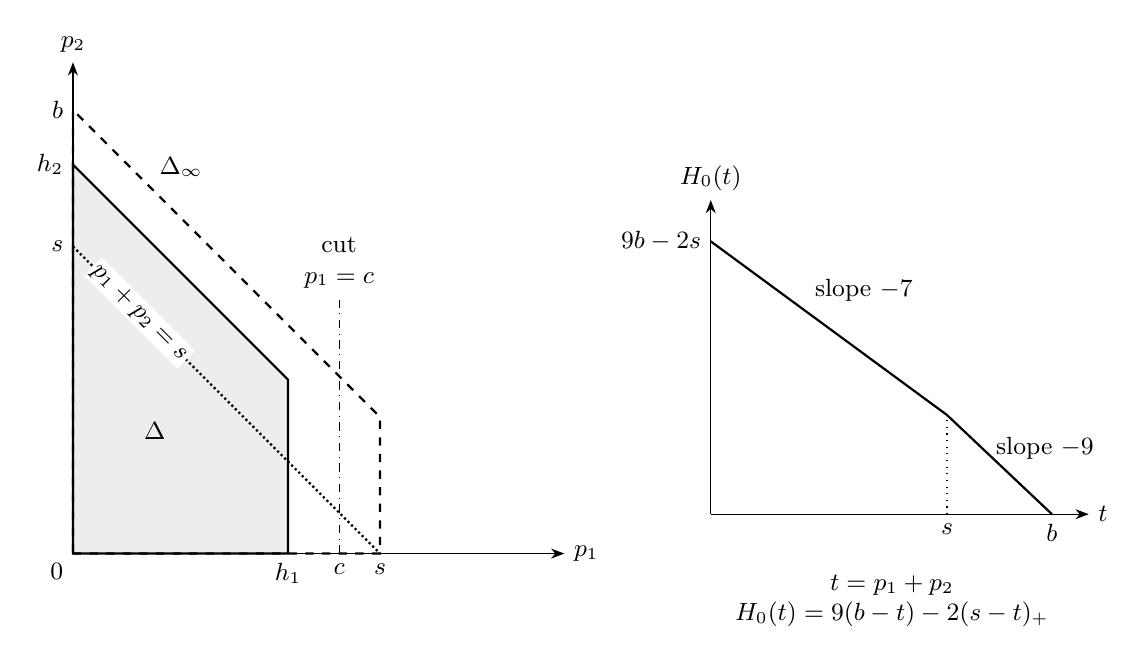
\begin{tikzpicture}[font=\small,>=Stealth]
 \begin{scope}[x=13cm,y=13cm]
  \fill[black!7] (0,0)--(.21,0)--(.21,.17)--(0,.38)--cycle;
  \draw[dashed,thick] (0,0)--(.3,0)--(.3,.133333)--(0,.433333)--cycle;
  \draw[thick] (0,0)--(.21,0)--(.21,.17)--(0,.38)--cycle;
  \draw[densely dotted,thick] (0,.3)--(.3,0);
  \draw[dash dot] (.26,0)--(.26,.25)
    node[above,align=center] {cut\\\(p_1=c\)};
  \draw[->] (0,0)--(.48,0) node[right] {\(p_1\)};
  \draw[->] (0,0)--(0,.48) node[above] {\(p_2\)};
  \node[below left] at (0,0) {\(0\)};
  \node[left] at (0,.433333) {\(b\)};
  \node[left] at (0,.38) {\(h_2\)};
  \node[left] at (0,.3) {\(s\)};
  \node[below] at (.21,0) {\(h_1\)};
  \node[below] at (.26,0) {\(c\)};
  \node[below] at (.3,0) {\(s\)};
  \node at (.08,.12) {\(\Delta\)};
  \node[above right] at (.075,.358333) {\(\Delta_\infty\)};
  \node[rotate=-45,fill=white,inner sep=1pt] at (.065,.235)
    {\(p_1+p_2=s\)};
 \end{scope}
 \begin{scope}[shift={(8.1cm,.5cm)},x=10cm,y=1.05cm]
  \draw[->] (0,0)--(.48,0) node[right] {\(t\)};
  \draw[->] (0,0)--(0,3.8) node[above] {\(H_0(t)\)};
  \draw[thick] (0,3.3)--(.3,1.2)--(.433333,0);
  \draw[dotted] (.3,0)--(.3,1.2);
  \node[left] at (0,3.3) {\(9b-2s\)};
  \node[below] at (.3,0) {\(s\)};
  \node[below] at (.433333,0) {\(b\)};
  \node[above right] at (.12,2.46) {slope \(-7\)};
  \node[right] at (.35,.8) {slope \(-9\)};
  \node[align=center] at (.23,-1.05)
    {\(t=p_1+p_2\)\\
     \(H_0(t)=9(b-t)-2(s-t)_+\)};
 \end{scope}
\end{tikzpicture}
\caption{The six-dimensional packing domain and its limiting base area.
The solid domain \(\Delta\) lies entirely below the cut \(p_1=c\).
The dashed domain \(\Delta_\infty\) is used to compute the limiting
volume \((1-a^3)/6\). The dotted line marks the change of slope of
\(H_0\); the portion of \(\Delta\) below it remains in the packing domain.
Each of the two marked points of the elliptic base contributes the
subtracted mass \((s-t)_+\). The drawing illustrates
\(h_1<c<s<h_2<b\); the full parameter order is
\eqref{six:truncation}.}
\label{fig:sixdim-moment}
\end{figure}

Such choices are possible by \eqref{six:auxiliary},
\eqref{six:volume}, and convergence of these domains to
\(\Delta_\infty\).  The cap supports are already wholly
inside every sufficiently close truncation.

The hypotheses of Lemma~\ref{surf:packing} hold.
First, \(H_0\) is positive on \(\Delta\).
As a function of \(t=p_1+p_2\), its slopes are \(-7\)
for \(t<s\) and \(-9\) for \(t>s\), so it is concave.
Each negative cap is concave as well, proving concavity
of \(P\).
The auxiliary simplices lie strictly away from the two
outer faces.  Choose \(\tau<1\) with
\(\tau h_1>\max_i r_i\) and \(\tau h_2>\max_i r_i\).
If \(p\notin\tau\Delta\), either
\(p_1>\tau h_1\) or \(p_1+p_2>\tau h_2\); in either case
all caps vanish.  Thus \(P=H_0\) there, with a uniform
positive lower bound.  We have used the concave limiting
density \(H_0\) throughout; only the model's integrated
areas are approximated by bordered pieces.

Construct the cubic family with the chosen \(d_1,d_2\).
Remove from its base \(C\) the marked points and all
intersections with \(\ell\cup Q\).  The remaining curve
has genus one and admits connected bordered exhaustions
of genus one.  Lemma~\ref{six:toric-model} supplies the
models \eqref{six:surface-form}, with uniform limiting
area \(H_0\), over these exhaustions.
Lemma~\ref{surf:packing} therefore embeds disjoint closed
balls of capacities \(R_i<r_i\), \(1\le i\le k\), compactly
in one such model, with neighborhood embeddings.
The entire chosen model has \(p_1\le h_1<c\), is away
from the double locus, and avoids the inverse images
of \(\ell\cup Q\) under the map to the plane.

Transfer this compact region into a nearby fiber
\(\widehat V\).  Lemma~\ref{six:moment-transfer} keeps it
below \(p_1<c\) and preserves the stated avoidance.
Apply the cut of Lemma~\ref{six:cut}.  The balls now lie
in \(Y\) off infinity and off the two forbidden vertical
submanifolds over \(D\cap E\) and \(D\cap H_\infty\).
The cut form is invariant and is in exactly the
polarization class of Lemma~\ref{six:quadric}.

Use Proposition~\ref{geo:transfer} for the first normal-cone
degeneration.  The allowed relative Moser identification
of Lemma~\ref{geo:relative-moser} preserves infinity and
the two disjoint forbidden vertical submanifolds.
It follows that the compact packing transfers into
\(T\setminus(E\cup H_\infty)\), with a Kähler form in
class \(H-aE\).  Lemma~\ref{geo:shell}, using relative
Moser for the disjoint divisors \(E,H_\infty\), identifies
this complement symplectically with
\[
 \left\{z\in\C^3:
          a<\pi\sum_{j=1}^3|z_j|^2<1\right\}.
\]
Add the central closed ball of capacity \(R_0<a\).
It is disjoint from all these compact shell balls, and
every source lies inside the open target.  Each operation
was defined on a neighborhood of the relevant compact
set; restricting these neighborhoods if necessary gives
the required neighborhood embeddings of the closed balls.
\end{proof}

\section{Completion of the packing theorem}\label{app:completion}

\begin{proof}[Sufficiency in Theorem~\ref{intro:main}]
Normalize the target capacity to one as in Section~\ref{intro:section}.
The case of one ball is immediate. If every requested capacity is
strictly less than \(1/2\), apply Proposition~\ref{app:small}.

Otherwise the strict pairwise inequalities imply that exactly one
requested capacity, say \(A\), is at least \(1/2\). All the inequalities
required by Proposition~\ref{app:large}, for \(n\ge4\), or by
Proposition~\ref{six:large}, for \(n=3\), are precisely the assumed
volume and pairwise inequalities. The applicable proposition gives
the entire requested packing, with embeddings on neighborhoods of
the closed sources. This proves sufficiency, and hence the theorem.
\end{proof}

\begin{thebibliography}{24}

\bibitem{Biran1997}
P.~Biran,
\emph{Symplectic packing in dimension 4},
Geom. Funct. Anal. \textbf{7} (1997), 420--437.
\href{https://doi.org/10.1007/s000390050014}{doi:10.1007/s000390050014}.

\bibitem{Biran1999}
P.~Biran,
\emph{A stability property of symplectic packing},
Invent. Math. \textbf{136} (1999), 123--155.
\href{https://doi.org/10.1007/s002220050306}{doi:10.1007/s002220050306}.

\bibitem{Biran2001}
P.~Biran,
\emph{Lagrangian barriers and symplectic embeddings},
Geom. Funct. Anal. \textbf{11} (2001), no.~3, 407--464.
\href{https://doi.org/10.1007/PL00001678}{doi:10.1007/PL00001678}.

\bibitem{BurnsGuillemin2004}
D.~Burns and V.~Guillemin,
\emph{Potential functions and actions of tori on K\"ahler manifolds},
Comm. Anal. Geom. \textbf{12} (2004), no.~1--2, 281--303.
\href{https://doi.org/10.4310/CAG.2004.v12.n1.a13}
{doi:10.4310/CAG.2004.v12.n1.a13}.

\bibitem{BurnsGuilleminLerman2002}
D.~Burns, V.~Guillemin, and E.~Lerman,
\emph{K\"ahler cuts},
Preprint, 2002.
\href{https://arxiv.org/abs/math/0212062}{arXiv:math/0212062}.

\bibitem{BuseHind2011}
O.~Buse and R.~Hind,
\emph{Symplectic embeddings of ellipsoids in dimension greater than four},
Geom. Topol. \textbf{15} (2011), 2091--2110.
\href{https://doi.org/10.2140/gt.2011.15.2091}{doi:10.2140/gt.2011.15.2091}.

\bibitem{BuseHind2013}
O.~Buse and R.~Hind,
\emph{Ellipsoid embeddings and symplectic packing stability},
Compos. Math. \textbf{149} (2013), 889--902.
\href{https://doi.org/10.1112/S0010437X12000826}{doi:10.1112/S0010437X12000826}.

\bibitem{BuseHindOpshtein2016}
O.~Buse, R.~Hind, and E.~Opshtein,
\emph{Packing stability for symplectic 4-manifolds},
Trans. Amer. Math. Soc. \textbf{368} (2016), 8209--8222.
\href{https://doi.org/10.1090/tran/6802}{doi:10.1090/tran/6802}.

\bibitem{EdtmairPerfectness2025}
O.~Edtmair,
\emph{Smooth perfectness of Hamiltonian diffeomorphism groups},
Preprint, 2025.
\href{https://arxiv.org/abs/2509.16327v1}{arXiv:2509.16327v1}.

\bibitem{EdtmairPacking2025}
O.~Edtmair,
\emph{Packing stability and the subleading asymptotics of symplectic Weyl laws},
Preprint, 2025.
\href{https://arxiv.org/abs/2509.15390v1}{arXiv:2509.15390v1}.

\bibitem{Fulton1998}
W.~Fulton,
\emph{Intersection Theory},
2nd ed., Springer-Verlag, 1998.
\href{https://doi.org/10.1007/978-1-4612-1700-8}
{doi:10.1007/978-1-4612-1700-8}.

\bibitem{FultonMacPhersonSottileSturmfels1995}
W.~Fulton, R.~MacPherson, F.~Sottile, and B.~Sturmfels,
\emph{Intersection theory on spherical varieties},
J. Algebraic Geom. \textbf{4} (1995), no.~1, 181--193.
\href{https://franksottile.github.io/research/pdf/spherical.pdf}
{Author manuscript}.

\bibitem{Gromov1985}
M.~Gromov,
\emph{Pseudo holomorphic curves in symplectic manifolds},
Invent. Math. \textbf{82} (1985), 307--347.
\href{https://doi.org/10.1007/BF01388806}{doi:10.1007/BF01388806}.

\bibitem{Hartshorne1977}
R.~Hartshorne,
\emph{Algebraic Geometry},
Graduate Texts in Mathematics, vol.~52,
Springer-Verlag, New York, 1977.
\href{https://doi.org/10.1007/978-1-4757-3849-0}
{doi:10.1007/978-1-4757-3849-0}.

\bibitem{Lazarsfeld2004}
R.~Lazarsfeld,
\emph{Positivity in Algebraic Geometry I:
Classical Setting: Line Bundles and Linear Series},
Ergebnisse der Mathematik und ihrer Grenzgebiete, 3.~Folge, vol.~48,
Springer-Verlag, Berlin--Heidelberg, 2004.
\href{https://doi.org/10.1007/978-3-642-18808-4}
{doi:10.1007/978-3-642-18808-4}.

\bibitem{Lerman1995}
E.~Lerman,
\emph{Symplectic cuts},
Math. Res. Lett. \textbf{2} (1995), no.~3, 247--258.
\href{https://doi.org/10.4310/MRL.1995.v2.n3.a2}
{doi:10.4310/MRL.1995.v2.n3.a2}.

\bibitem{McDuffPolterovich}
D.~McDuff and L.~Polterovich,
\emph{Symplectic packings and algebraic geometry},
Invent. Math. \textbf{115} (1994), 405--429.
\href{https://doi.org/10.1007/BF01231766}{doi:10.1007/BF01231766}.

\bibitem{Moser1965}
J.~Moser,
\emph{On the volume elements on a manifold},
Trans. Amer. Math. Soc. \textbf{120} (1965), no.~2, 286--294.
\href{https://doi.org/10.1090/S0002-9947-1965-0182927-5}
{doi:10.1090/S0002-9947-1965-0182927-5}.

\bibitem{Opshtein2013}
E.~Opshtein,
\emph{Singular polarizations and ellipsoid packings},
Int. Math. Res. Not. \textbf{2013} (2013), no.~11, 2568--2600.
\href{https://doi.org/10.1093/imrn/rns137}{doi:10.1093/imrn/rns137}.

\bibitem{SchlenkFolding}
F.~Schlenk,
\emph{On symplectic folding},
Preprint, 1999.
\href{https://arxiv.org/abs/math/9903086}{arXiv:math/9903086}.

\bibitem{SchlenkBook}
F.~Schlenk,
\emph{Embedding Problems in Symplectic Geometry},
de Gruyter Expositions in Mathematics, vol.~40,
Walter de Gruyter, Berlin, 2005.
\href{https://doi.org/10.1515/9783110199697}{doi:10.1515/9783110199697}.

\bibitem{SchlenkHand}
F.~Schlenk,
\emph{Packing symplectic manifolds by hand},
J. Symplectic Geom. \textbf{3} (2005), no.~3, 313--340.
\href{https://doi.org/10.4310/JSG.2005.v3.n3.a1}{doi:10.4310/JSG.2005.v3.n3.a1}.

\bibitem{SiegelYao2025}
K.~Siegel and Y.~Yao,
\emph{On symplectic packing problems in higher dimensions},
Math. Ann. \textbf{392} (2025), 5361--5392.
\href{https://doi.org/10.1007/s00208-025-03221-7}
{doi:10.1007/s00208-025-03221-7}.

\bibitem{Stacks}
The Stacks project authors,
\emph{The Stacks project}, 2026.
\url{https://stacks.math.columbia.edu}.

\bibitem{Traynor}
L.~Traynor,
\emph{Symplectic packing constructions},
J. Differential Geom. \textbf{41} (1995), no.~3, 735--751.
\href{https://doi.org/10.4310/jdg/1214456483}{doi:10.4310/jdg/1214456483}.

\bibitem{WittNystrom2024}
D.~Witt Nystr\"om,
\emph{Deformations of K\"ahler manifolds to normal bundles and
restricted volumes of big classes},
J. Differential Geom. \textbf{128} (2024), no.~3, 1177--1223.
\href{https://doi.org/10.4310/jdg/1729092457}
{doi:10.4310/jdg/1729092457}.

\end{thebibliography}

\end{document}
